\documentclass[12pt]{article}
\usepackage{amsmath}
\usepackage{graphicx}
\usepackage{fancyhdr}
\usepackage[margin=1in]{geometry}
\usepackage{url}
\usepackage{float}
\usepackage{todonotes}
\usepackage{fixltx2e}
\usepackage{gensymb}
\usepackage{enumitem}
\usepackage{textpos}
\usepackage{appendix}
\usepackage{color}
\usepackage{tabu}
\usepackage{listings,xcolor}
\usepackage{pdflscape}
\usepackage{longtable}
\usepackage{multirow}
\usepackage{textcomp}
\usepackage{pdfpages}
\usepackage{enumitem}
\usepackage{wrapfig}
\usepackage{array}
% to bold row of table
\newcolumntype{$}{>{\global\let\currentrowstyle\relax}}
\newcolumntype{^}{>{\currentrowstyle}}
\newcommand{\rowstyle}[1]{\gdef\currentrowstyle{#1}%
  #1\ignorespaces
}
\usepackage{libertine} \usepackage[libertine]{newtxmath}
\newcolumntype{L}{>{\arraybackslash}m{5in}}
\setlength\extrarowheight{2pt}
\pagestyle{fancy}
\usepackage[font=small,labelfont=bf,tableposition=top]{caption}
\fancyhf{}
% Header and footer
\fancyhead[L]{ENGR 4595}
\fancyhead[C]{Final Report}
\fancyhead[R]{Group 2}
\fancyfoot[R]{Page \thepage}
\renewcommand{\headrulewidth}{0.4pt}
\renewcommand{\footrulewidth}{0.4pt}
\newcommand*{\everymodeprime}{\ensuremath{\prime}}
\begin{document}
\begin{titlepage}

\newcommand{\HRule}{\rule{\linewidth}{0.5mm}} % Defines a new command for the horizontal lines, change thickness here

\center % Center everything on the page
 
%----------------------------------------------------------------------------------------
%	HEADING SECTIONS
%--------------------------------------------------------------------s--------------------

\textsc{\LARGE Laurentian University}\\[1.5cm] % Name of your university/college
\textsc{\Large Capstone}\\[0.5cm] % Major heading such as course name
\textsc{\large ENGR-4595}\\[0.5cm] % Minor heading such as course title

%----------------------------------------------------------------------------------------
%	TITLE SECTION
%----------------------------------------------------------------------------------------

\HRule \\[0.4cm]
{ \huge \bfseries Final Report: Robot Drive System Redesign}\\[0.4cm] % Title of your document
\HRule \\[1.5cm]
 
%----------------------------------------------------------------------------------------
%	AUTHOR SECTION
%----------------------------------------------------------------------------------------

\begin{minipage}{0.4\textwidth}
\begin{flushleft} \large
\emph{Submitted by Group 2:}\\
Dyson Chambers \textsc{} \\
Dominic Girard \textsc{} \\
Christopher Gravelle \textsc{} \\
Jacob Lachapelle \textsc{} \\
Genevi\`{e}ve Rodrigue \textsc{}
\end{flushleft}
\end{minipage}
~
\begin{minipage}{0.4\textwidth}
\begin{flushright} \large
\emph{For project client:} \\
Penguin ASI\\
Regional Road 55\\
Naughton, ON % Supervisor's Name
\end{flushright}
\end{minipage}\\[4cm]


% If you don't want a supervisor, uncomment the two lines below and remove the section above
%\Large \emph{Author:}\\
%John \textsc{Smith}\\[3cm] % Your name

%----------------------------------------------------------------------------------------
%	DATE SECTION
%----------------------------------------------------------------------------------------

{\large April 26, 2016}\\[3cm] % Date, change the \today to a set date if you want to be precise

%----------------------------------------------------------------------------------------
%	LOGO SECTION
%----------------------------------------------------------------------------------------

%\includegraphics{Logo}\\[1cm] % Include a department/university logo - this will require the graphicx package
 
%----------------------------------------------------------------------------------------

\vfill % Fill the rest of the page with whitespace
\end{titlepage} 

% front matter goes here
\tableofcontents
\newpage
\listoftables
\newpage
\listoffigures
\newpage
% body material goes here
\section{Introduction}
Penguin ASI is a robotics firm engaged in the development of automation strategies for the mining industry and the development of telerobotic systems to work in extreme and hazardous environments. As the use of automated technology becomes more prevalent in the mining industry there comes a need to develop a telecommunications network. In order to prevent the need to retrofit an existing mine with a communications network, Penguin had developed an optical communications range extender and mounted it on a teleoperated, mobile platform to be able to relay the signals. The first iteration of this platform had some issues with its design that Penguin had wished to resolve in a second iteration prototype. In order to produce a functional prototype all issues with the previous version must have been addressed, and the robot must have been able to achieve certain functional requirements laid out by the client, Penguin ASI.  
\subsection{Problem Statement}
The initial communications robot produced by Penguin ASI had displayed many issues affecting its performance that needed to be addressed. Its operating environment was intended to include traversal through wet and rough terrain, which required all drive components to be sealed against water and dirt. To seal the original drive boxes gasket maker was used, but proved to be inadequate and allowed water to enter the drive box as seen in Figure~\ref{fig:inside_drive_box_orig}. Secondly, the drive box travel was not limited to $\pm$30\degree rotation initially, and a spring system was implemented as a temporary solution. Only two, 746\,W motors were used, and after testing were deemed insufficient to drive the vehicle and payload up hills of a 20\% grade. Furthermore, each motor drove four wheels and transmitted power through a long chain extending the length of the vehicle as seen in Figure~\ref{fig:interior_orig}. The length and complexity of the chain driven system introduced many modes of failure, slapped the bottom of the vehicle during skid steer operation and change of direction, and did not have an adequate tensioning device. 
\begin{figure}[h]
\centering
\begin{minipage}{0.45\linewidth}
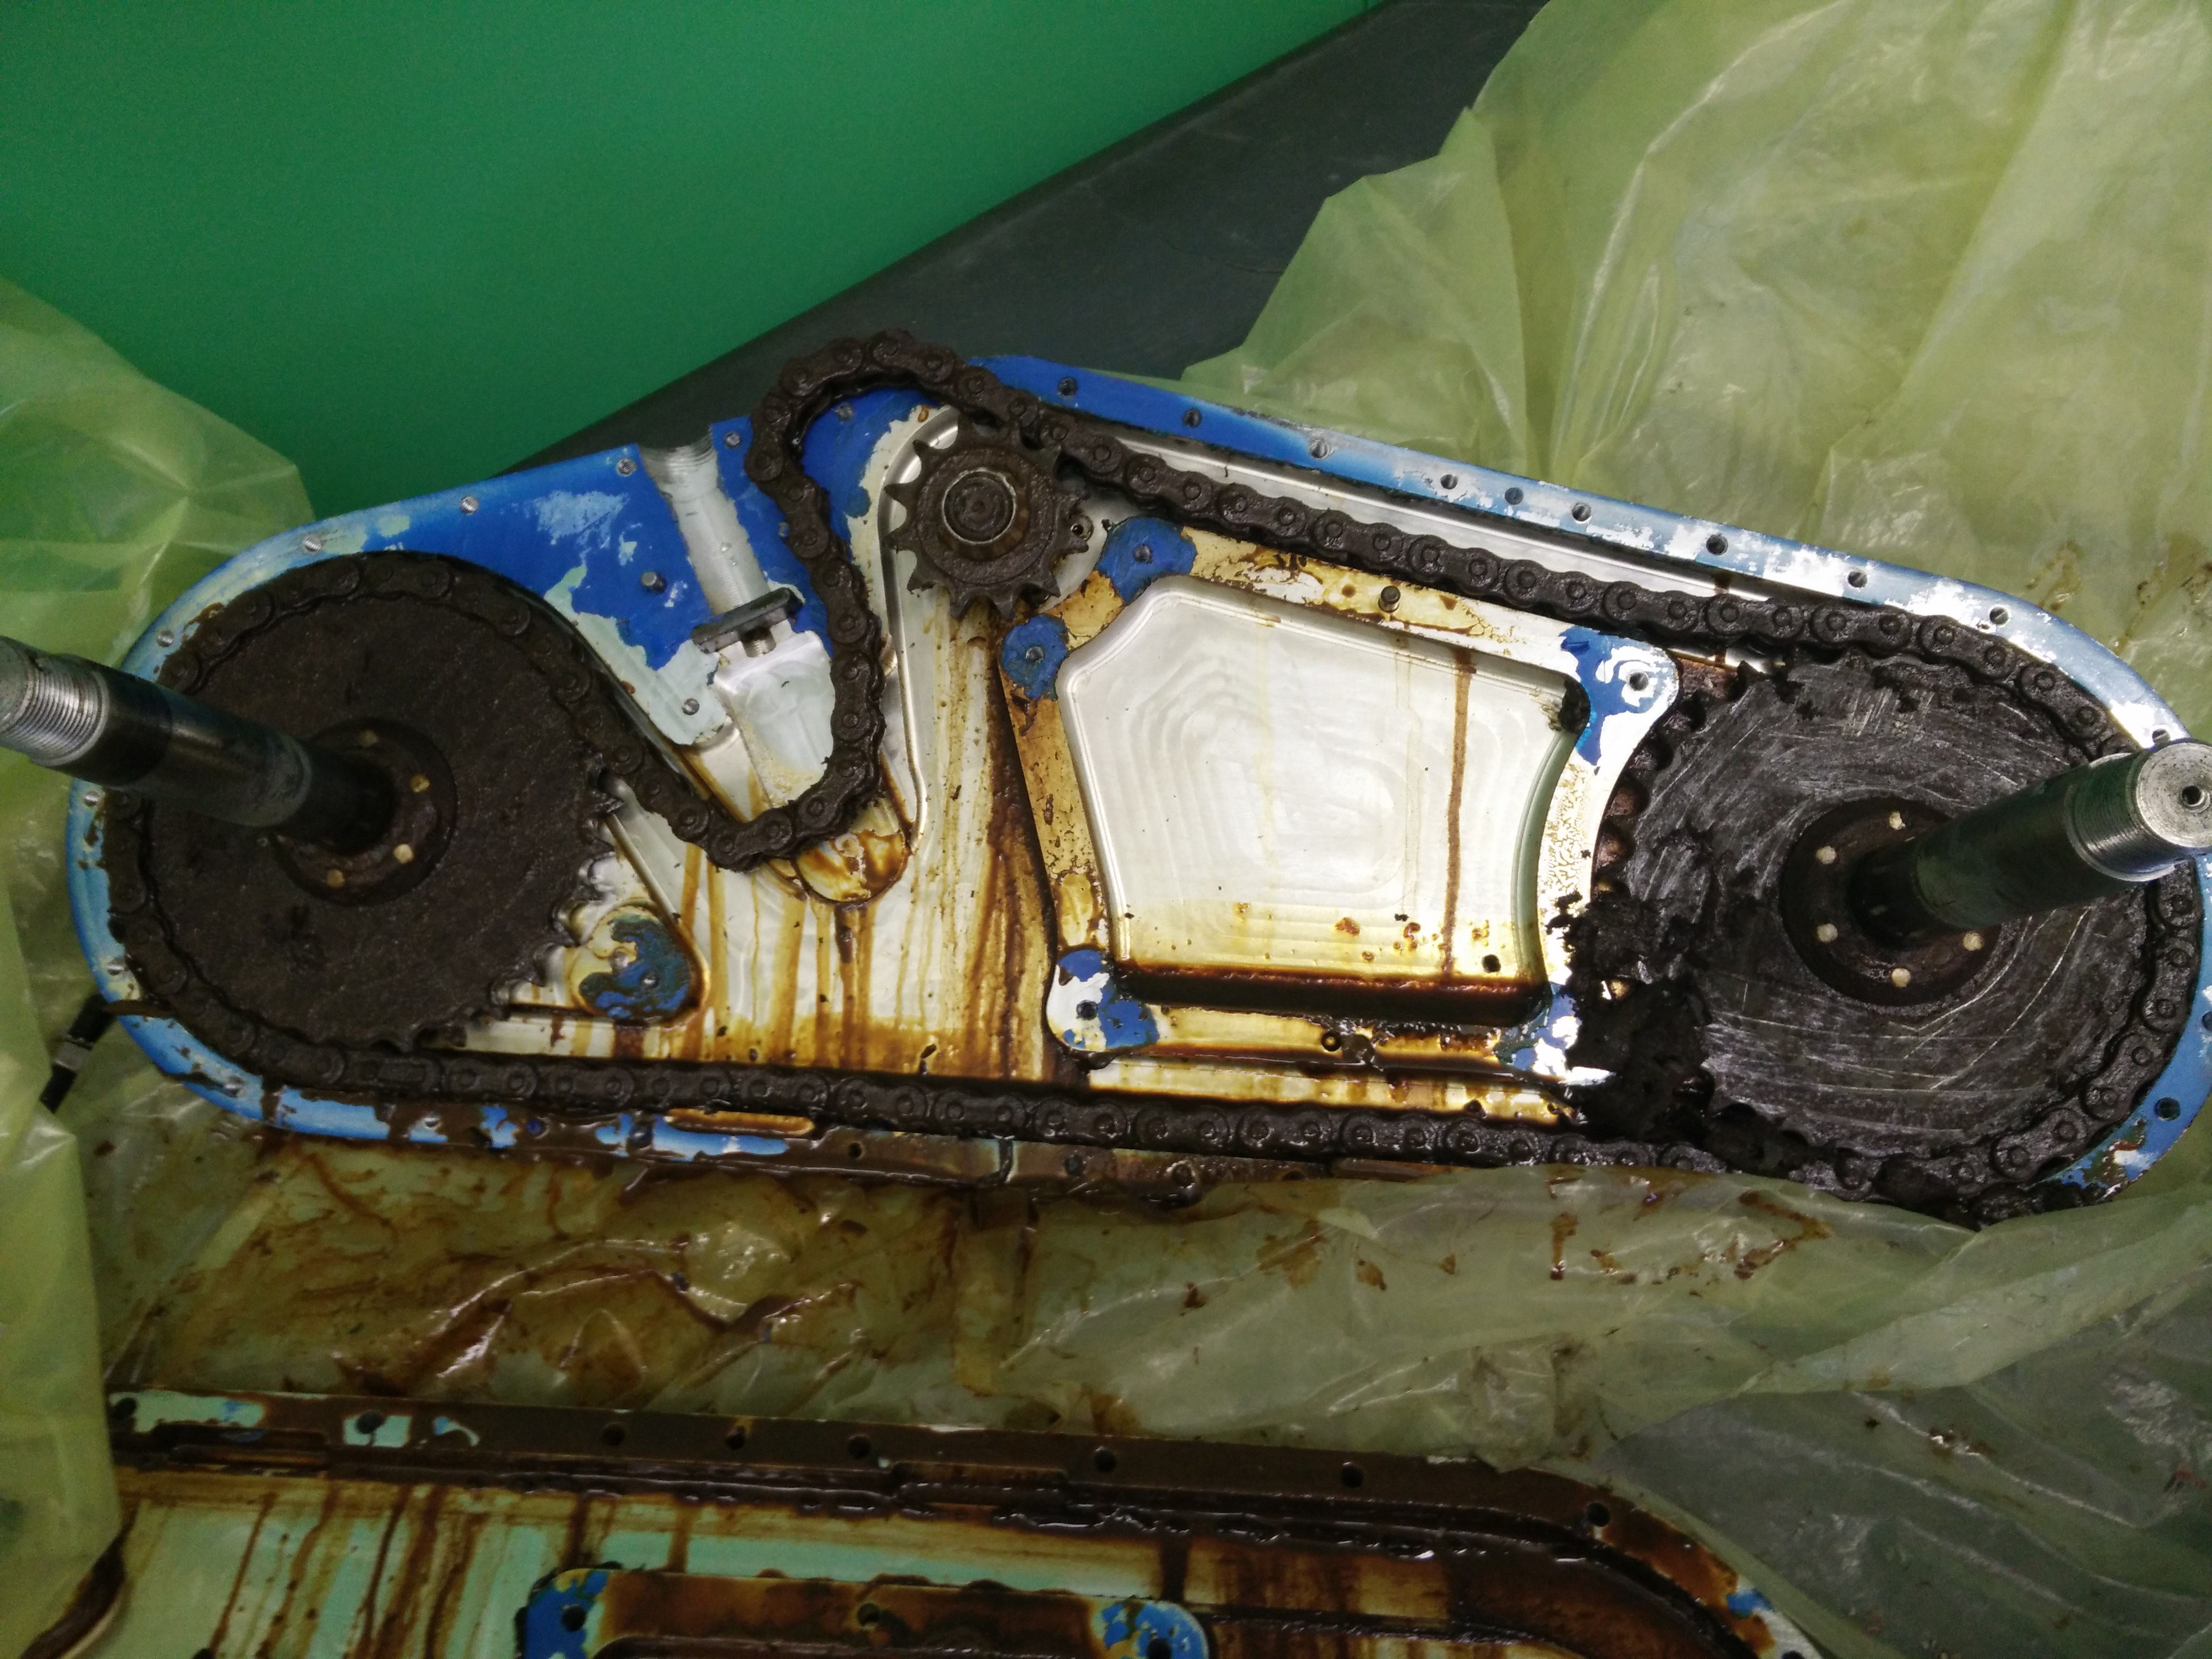
\includegraphics[width=\linewidth]{./images/inside_drive_box_orig}
\caption{Original Drive Box Interior Demonstrating Improper Sealing}
\label{fig:inside_drive_box_orig}
\end{minipage}
\begin{minipage}{0.45\linewidth}
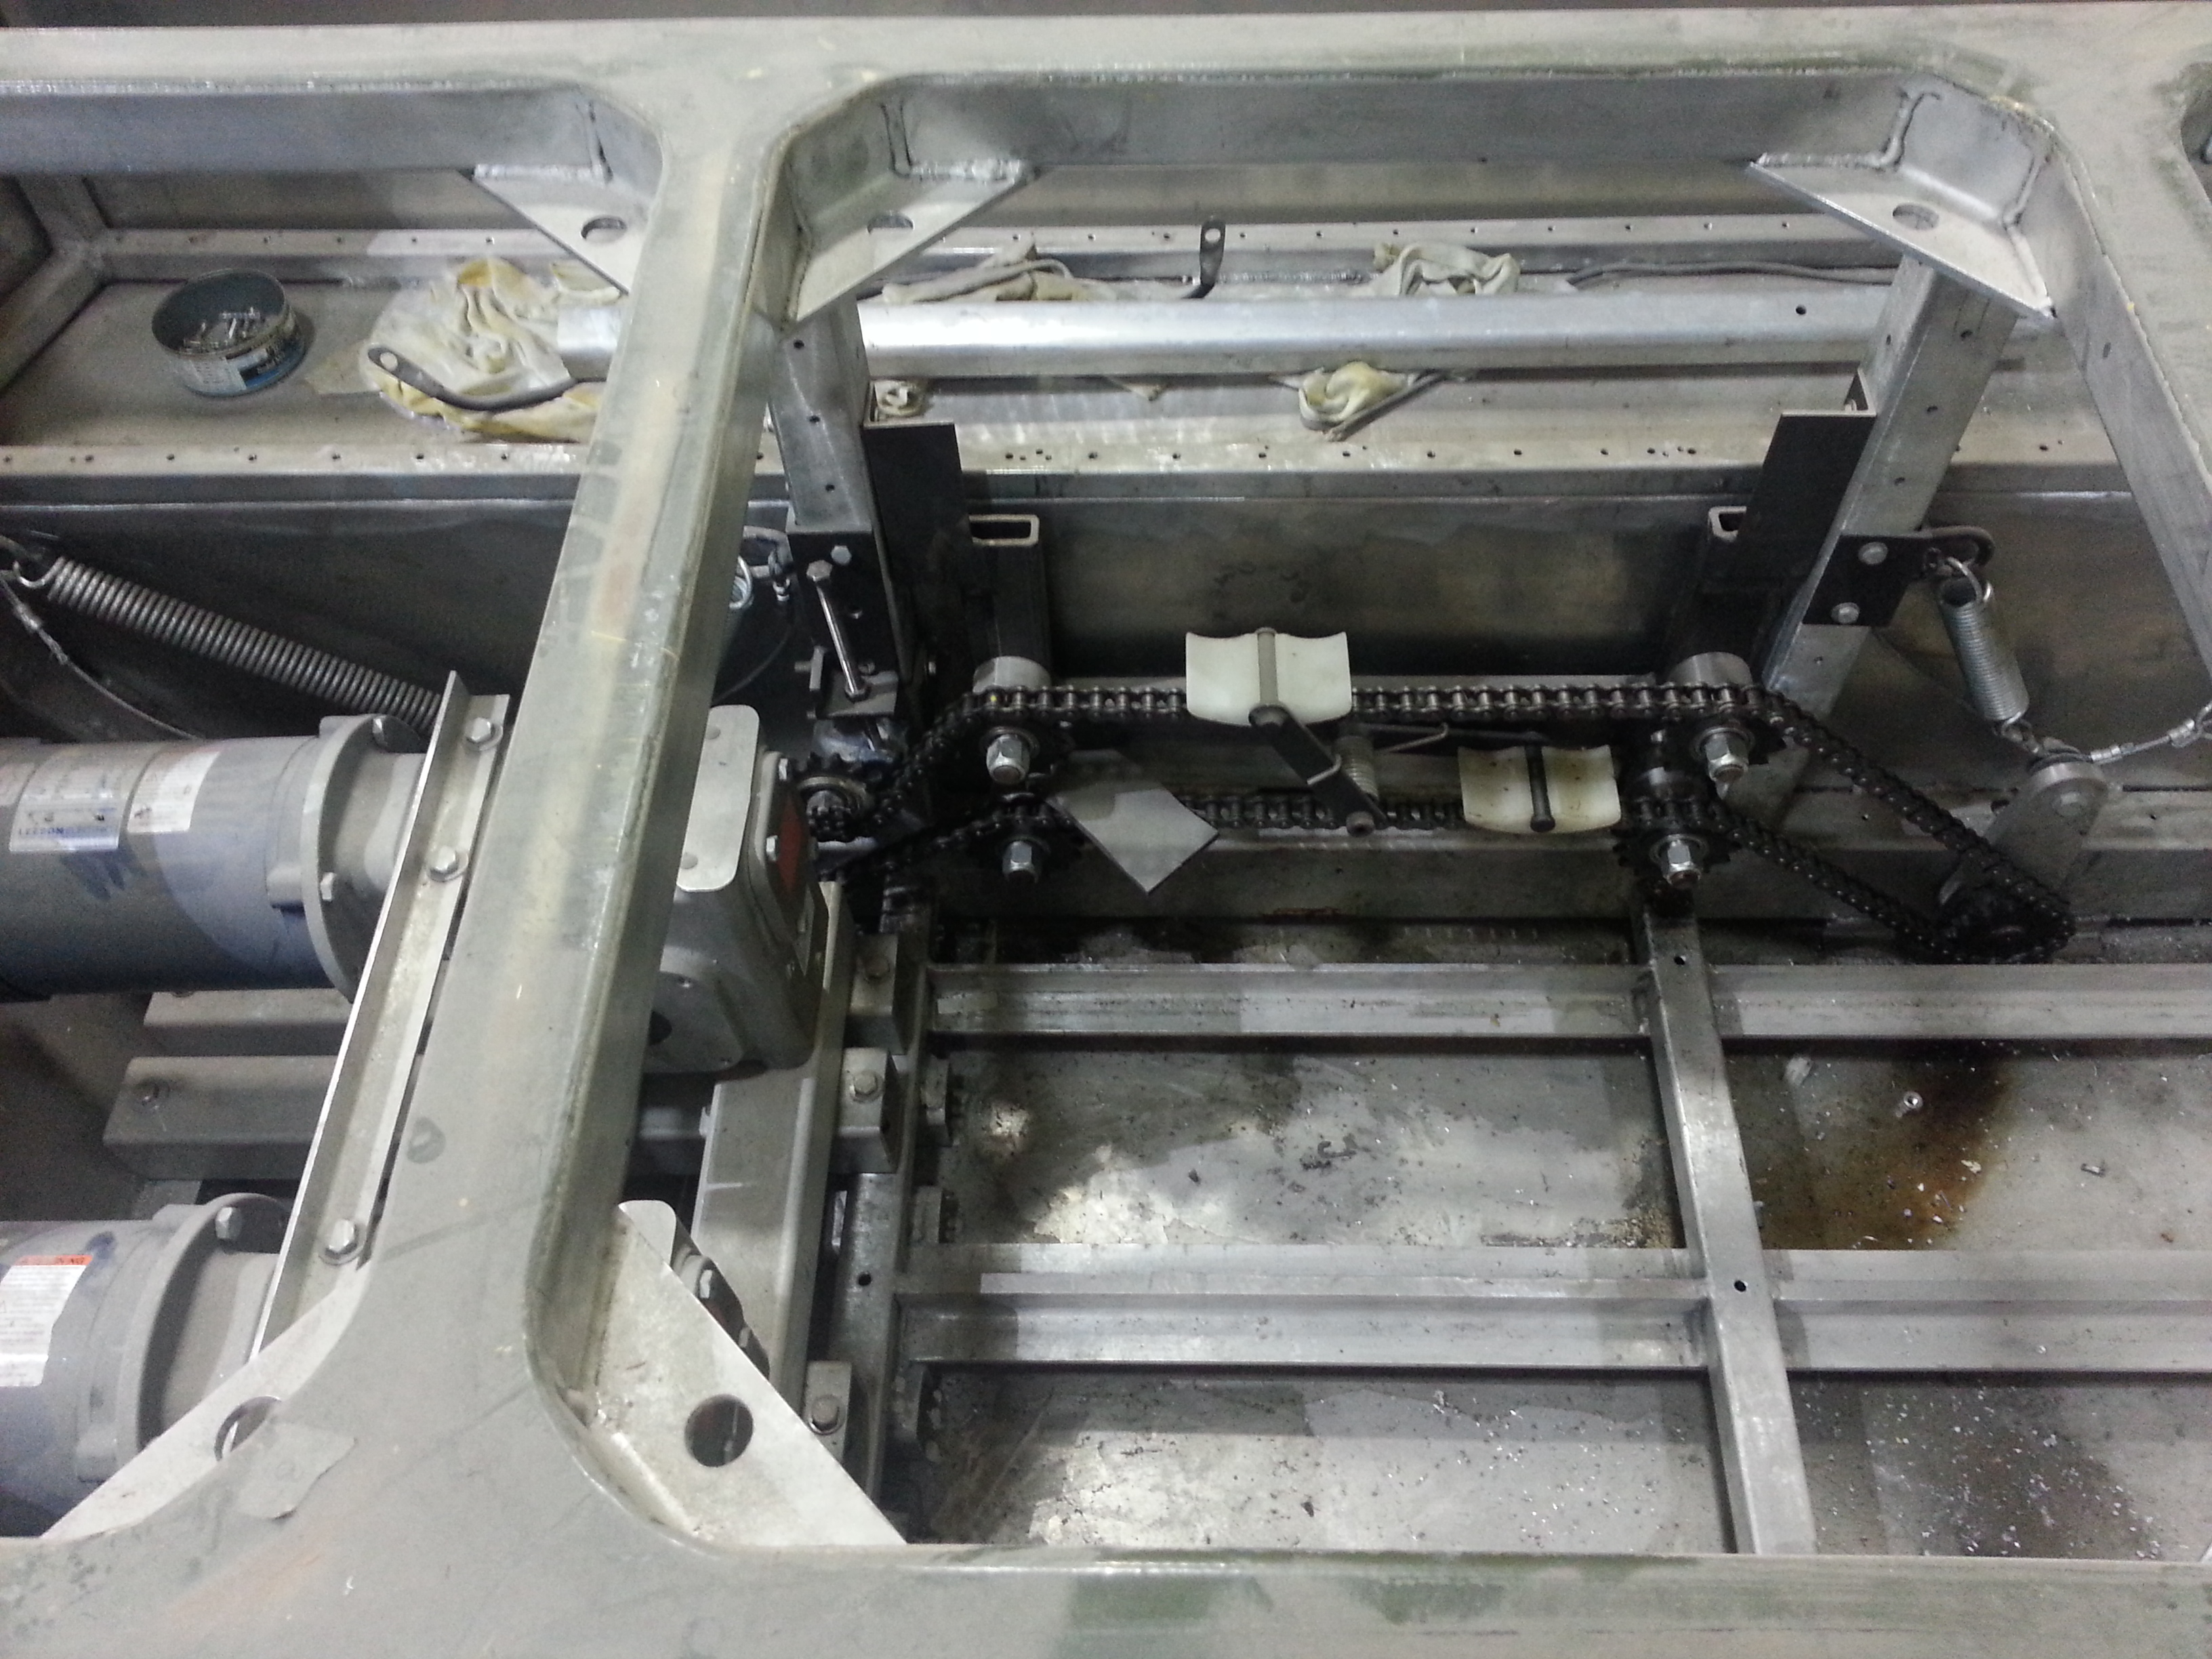
\includegraphics[width=\linewidth]{./images/interior_orig}
\caption{Chain Driven System Inside Vehicle Body}
\label{fig:interior_orig}
\end{minipage}
\end{figure}

The disassembly of the original driveboxes was difficult and it was observed that there was no way to determine oil levels without opening them up. Also, under skid steer operation it was reported that the drive boxes underwent significant deflection which was not desireable. Each drive box was chain driven, however there was no method to determine the chain tension, which was problematic and was suspected to be the cause of premature failure of chains. Other components that were failing included radial bearings used on the drive shafts and wheel shafts. After opening the drive boxes it was observed that these radial bearings were paired with a single taper roller bearing and it was suspected that the cause of failure was the axial loading on the radial bearing. 
\subsection{Functional Requirements}
Overall the vehicle was able to drive and maneuvre with limited capabilities, however it was in the interest of the client to address these issues for a redesign of the product. In order to meet the needs of the client a list of requirements for the final design were agreed upon. The requirements were broken down into six main categories, with each highlighting the necessary functionality for the redesign of the communications robot. 
\subsubsection{Power}
The vehicle was to be fully battery powered using six EV Traction Dry Cell Industrial Battery Blocks. To drive the vehicle, four 746\,W DC motors were provided by Penguin ASI. The drive time of the vehicle was to exceed one hour at peak operating conditions, and the batteries were to be seated in the vehicle to provide clearance between battery terminals and frame components.
\subsubsection{Operating Conditions}
The vehicle was to be used in aboveground and underground mining applications, and as such would be subject to varying temperatures, however the client had specified the need to operate primarily in 2\,\degree C. The vehicle also needed to be able to climb and descend a maximum grade of 20\% and have every component sealed from external water.
\subsubsection{Size and Weight}
All components of the vehicle were to remain within the dimensions of the frame with the exception of the wheels. The robot needed to be able to carry a payload of 230\,kg in addition to its own weight, and be able to reach a top speed of 3\,km/h under these conditions.
\subsubsection{Interfacing}
Penguin ASI had specified the need to reuse the frame from the existing robot, however minor frame modification were permitted. Motor interfacing needed to be done using a Roboteq controller, and battery charging was to be carried out by employees at Penguin. The redesign of the vehicle needed to ensure that that existing communications devices and telescoping arms could still be mounted on the upper platform of the frame, and that space be left in the wings of the vehicle to accomodate electrical components.
\subsubsection{Robot Control}
The motors on each side of the vehicle were to be controlled independently. A Roboteq controller was to be used, and appropriate voltage limits were to be programmed into the controller to prevent damaging the motors. For testing purposes, the use of a laptop to and joystick to control the motors was permitted. The implementation of wireless control was to be carried out by Penguin employees upon the successful demonstration of an operable vehicle.
\subsubsection{Care and Maintenance}
All new components were to be designed with the intent of improving functionality and maintainability. It was desired that all components be easy to assemble/disassemble, internal components be easily accessible, and grease nipples be incorporated to grease bearings. Furthermore, a means to check belt tension was to be incorporated in the final design.       
\section {Design Alternatives}
The main feature to the project was based off of power transmission from the motors to the wheels. For this, three different methods were explored. 

\subsection{Chains}
The first consideration was a chain drive which was also found on the previous iteration of the robot. However, chains proved to require quite a bit of maintenance and must operate in a sealed and lubricated gearbox. Aside from sealing concerns, corrosion and stretching from use were other issues that posed problems and increased maintenance time. Many of these robots will be on standby and must be ready to use whenever needed, therefore any maintenance or checks require before every use are unfavorable. 

Chains did prove to have some advantages such as great operating efficiencies, being a cost efficient option and consisting of replacement parts that are readily available in most industrial settings.

\subsection{Shafts}
The second was a serial shaft configuration that would require many 90\degree joints which are expensive, bulky and are high maintenance as well. This option was nearly eliminated right off the hop but was kept for comparison and analysis in the decision making process. 

\subsection{Belts}
The third and final option was a synchronous belt drive system. After some research and discussions with the engineers at Gates, one of the world's leading manufacturers in belt systems, it was concluded that a belt drive would be very suitable for the application at hand. Operating in a dry gearbox, virtually no stretch over it's lifetime and a significant increase in longevity over a chain drive are all features that made belts much more attractive. Synchronous belts also have operating efficiencies similar to chains, thus making them just as viable. As claimed by Gates, belts are to last 3 times longer than chains and sprockets for belts are to last 10 times longer than ones for chains. It is to note that belt don't take side loading or twisting very well, therefore much emphasis on reducing these affects were a main focus in the design of the drivebox structure. Corrosion was also an important consideration for every option, and even though belts won't rust, other components such as the sprockets and shafts very well could. Some part sourcing revealed that aluminum sprockets could be purchased and other steel components could be sprayed with a durable, anti-rust coating that wouldn't contaminate the belt and bearings.

Belts were chosen after careful evaluation against the other alternatives as seen in the Pugh matrix in Appendix ~\ref{pugh}






\section{Project Management}

From the beginning, project management was an important tool used to keep our team working efficiently and on time  to be able too build and finish our proposed final design. Do to the inherent structure of the course, we added two main milestones, the design and build phase.The first haft of our semester was dedicated to designing our solution to the problem. During this time, we created a work schedule using WBS (Work Breakdown Structure) to get a better visual understanding of the scope and after created our initial Gantt chart. Since the first scope breakdown, the WBS and Gantt chart underwent many revision because of the fluctuating scope of work of our project kept adjusting to what would be reasonably possible to complete in the allocated amount of time. The final WBS can be found~\ref{fig:wbs] in Appendix~\ref{wbs}.

During the building phase, it became evident of the amount of work needed to finish the project. Milestones were set at many point to ensure that we kept on schedule. Our first major milestone was to get the first outer drive box completed to ensure that all designed components would fit and interact properly before creating the other drive boxes. After completion of the first drive box and implement minor changes for manufacturing ease, we then started our stretched goals which was completing all three other drive boxes. During both manufacturing phases of the drive boxes, one or two of our group members worked on the structural frame modification which ended up being one of the most times consuming area of the building phase. 

Critical documentation deadlines were also set as milestones. These reports and presentations were typically done nearing the end of the every phase. This had as advantage to include all current changes before submission of the documents and to have all necessary information to complete the report at once, instead of someone waiting on the information. 

Finally, our team spent hours on building and manufacturing. Our initial estimate of the time needed to complet the project was 182 hours on the CNC Lathe, 146 on the CNC mill and 61 hours on frame accommodation. This thus needed us to spend at a minimum 30 hours a week on manufacturing alone. In total, all member of the team gave 270 hours in manufacturing which is reflected in the Gantt chart. The final Gantt chart can be found~\ref{fig:gantt} in Appendix~\ref{gantt}.
\section{Final Design}
The final design of the robots drive system is very similar to the proposed design provided to Penguin ASI and Laurentian University in December. Using a belt drive over a chain drive was accepted through our proposal along with keeping it battery powered. In the final design the batteries used were ones that were provided by Penguin ASI. Four batteries were still required to power all four brush-less DC motors and two other batteries required to supply power to the other electronic components on board the robot. The final design also had features that were in the proposed design, such as removable interior components, easy serviceability and keeping it as a modular design. Having the components easily removable will allow anyone who is maintaining the drive system have access to all the bearings for re-greasing and easy vision for inspection of belts condition.  After assembling one exterior drive box, some small design changes were made that were not noticed in the CAD model assemblies or were notified to us from Penguin Employees after the proposal report had been submitted. None of these changes required the proposed design to drastically change but actually improved the overall design and reduced the amount of machining time required for some components. An example of reducing machining time would be the new hubs located at the back side do the drive boxes. In the proposed design the rear hubs required machining on both the exterior and interior, but with the new design all exterior machining was not required.Below is a table with the robots specifications.

The exploded view of assembly that can be seen in "FIGURE BELOW" shows how each individual drive box goes together along with its connection to the robots frame. All four motors sit inside the robot frame and are each coupled with a flexible Lovejoy coupling to the output shaft that rotates withing the pivot. The torque from the motor is then transfered through the output shaft and is then transmitted through the belt to two wheel shafts. Those wheel shafts each have a foam filled tire attached to the end with a tapered fit mount and a castle nut ensuring the mount doesn't not come off the tapered shaft mount.

\begin{comment}
	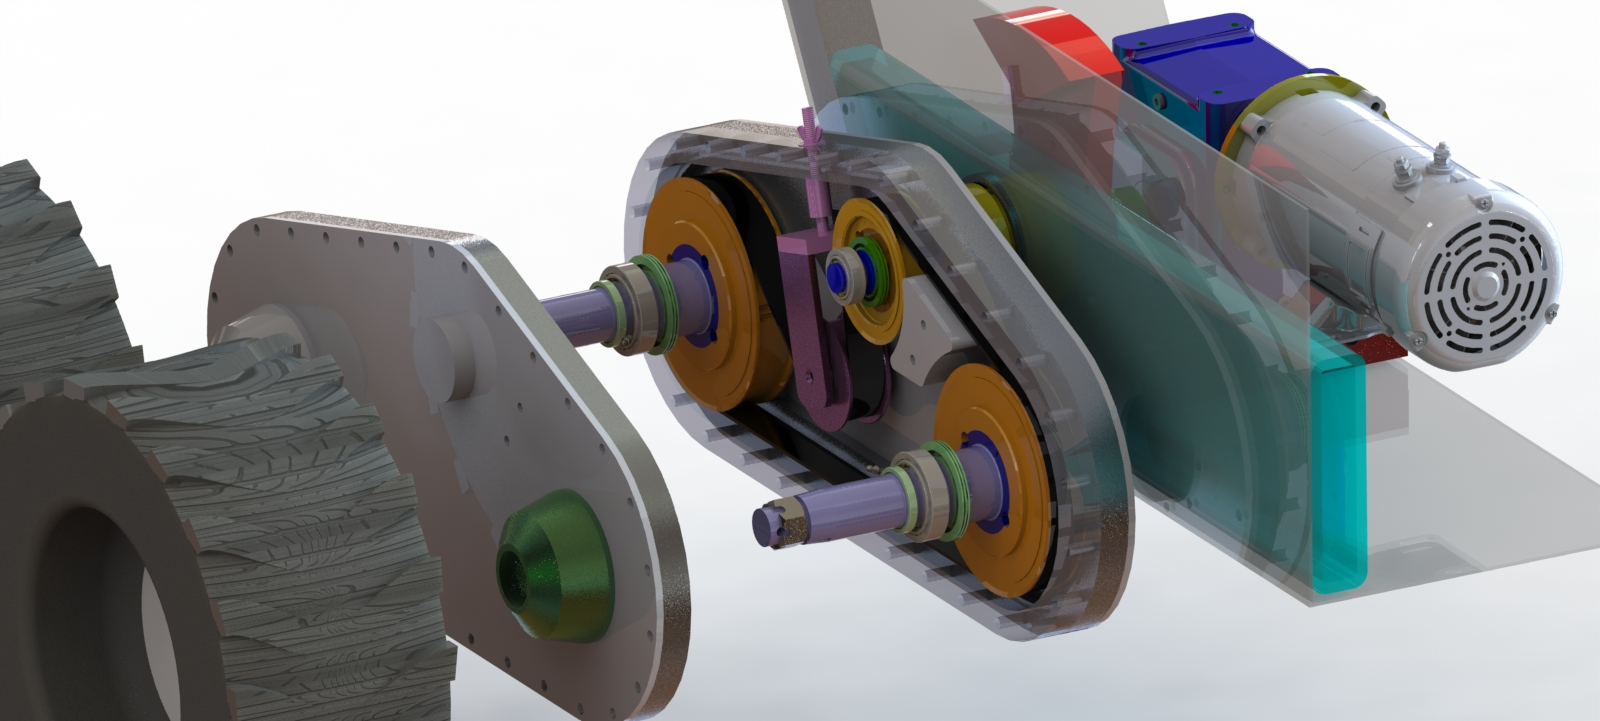
\includegraphics[width=\linewidth]{drive_box_presentation_rndr.jpg}
	\caption{Rendering showing one quarter of robot exterior drive assembly with front case frame and wheels off. }
	\label{fig:Assembly of quarter robot}
\end{comment}

What makes this design a more acceptable design over the previous design that Penguin ASI originally had is the simplicity of it. In their previous design their was only two motors used to power the four ex trier drive boxes, which required that two output shafts on one side had to share the output from one motor. In the new design each drive box will be getting its own motor to provide power and this reduces the amount of moving parts needed. Such as, a chain to allow each output shaft to be sharing one motor and tensions along that chain. Each component added arises a new point of possible failure during operation, so reducing the amount of moving parts also reduces this possibility. Another feature that the new design has over the old is the accessibility of the components inside the drive box for maintenance and repair if required. The new design gives you full access to all the interior components once the front case plate is removed. From this you can easily remove the wheel shafts and to remove the output shaft, only a set screw at the coupling is needed to be removed. All moving components can now be accessed easily and reduces the time required for an individual to work on. Using belts over chains reduces the maintenance cost, since belts do not require any lubrication and run in a dry casing.



\section{Loading Conditions}
As with any off road vehicle, it is always difficult to predict loading conditions as there is an infinite amount of scenarios due to the varying environment and terrain, however it can usually be generalized to a few simple, yet appropriate cases. Also, it is important for one to remind themselves what the vehicle is being designed for. Although it is an off-road vehicle, it is not designed for extreme conditions or dangerous scenarios. It's the same logic for someone who owns an economical car; they wouldn't be taking this vehicle into the bush through deep mud or rough terrain as it will most likely end up with broken parts. In this case, the robot is to be operated in a normal mining environment where the environment conditions are assumed to be a regular mining road built from crushed, roughly fist sized rock, and a max ramp grade of 20\% or incline of 11.3 degrees. Driving forward up a ramp and a skid steer turn on a ramp were then evaluated. As one could imagine, the skid steer motion when the robot is balancing on two, opposite diagonal wheels resulted in the highest forces, therefore these were used for analysis. With the weight distribution of the coupled wheels being 40/60, the 60\% wheel is used for analysis and its design is to be duplicated to the other wheel. The resulting forces are summarized in     
\\
 ***INSERT TABLE***
\\
It should be noted that only a static analysis was conducted for this project due to slow operating speeds. With a top speed of 3 km/h, the forces due to dynamic loading would only differentiate slightly. To compensate for this, a larger factor of safety was desired for each component. Given an adequate time line, one could conduct a full dynamic simulation to obtain more accurate results and confirm that the design to follow is indeed adequate for the imposed loading conditions. 

\section{Belt Drive}
\subsection{Description}
\subsection{Design Constraints}
\subsection{Functional Requirements}
\subsection{Alternate Solutions}
\subsection{Analysis and Design}

\section{Wheel Shaft Assembly}
\subsection{Description}
\subsection{Design Constraints}
\subsection{Functional Requirements}
\subsection{Alternate Solutions}
\subsection{Analysis and Design}
\subsubsection{Wheel Shaft}
\subsubsection{Wheel Bearings}
\subsubsection{Shaft Seals}
\subsubsection{Front Bearing Housings}
\subsubsection{Rear Bearing Housing}
\subsubsection{Rim Mount}


\section{Final Budget}
\begin{landscape}
\begin{longtable}{| $l^l^l^l^l^l^l |} 
\caption[Final budget for Parts]{Final Budget and lead times for purchased parts before taxes and shipping fees.}  \label{tab:budg_pur} \\
%\begin{tabular}{| $p{4cm}^p{3cm}^l^l^l^l^l |} 
\hline
Component & Manufacturer & Supplier & Price/Unit & Quantity & Total  & Lead time\\ \hline
\endfirsthead
\hline
Component & Manufacturer & Supplier & Price/Unit & Quantity & Total  & Lead time\\ \hline
\endhead
 \rowstyle{\bfseries}  Continued... &  &  &  &  &  & \\ \hline
\endfoot
\endlastfoot
Hub O-rings & DAE & BDI & \$0.23 & 8 & \$1.84 & Stock\\
Bearing Housing O-ring & DAE & BDI & \$0.35 & 16 & \$5.60 & Stock\\
Wheel Hub O-ring & DAE & BDI & \$0.35 & 8 & \$2.80 & Stock\\
Pivot O-ring & DAE & BDI & \$0.28 & 12 & \$3.36 & Stock\\
Drive box Custom O-ring & - & BDI & \$17.51 & 16 & \$280.16 & 4 Days\\
 &  &  &  &  &  & \\
Large Sprockets & Martin Sprocket & BDI & \$179.21 & 8 & \$1,433.68 & 4 to 5 Weeks\\
Small Sprockets & Martin Sprocket & BDI & \$101.29 & 4 & \$405.16 & Stock\\
Large Bushing For Sprocket & Martin Sprocket & BDI & \$20.00 & 8 & \$160.00 & Stock\\
Small Bushing For Sprocket & Martin Sprocket & BDI & \$16.31 & 4 & \$65.24 & Stock\\
Belt & Gates & BDI & \$125.00 & 4 & \$500.00 & Stock\\
 &  &  &  &  &  & \\
20 mm Sealed Ball Bearing & Amcan & BDI & \$20.17 & 8 & \$161.36 & Stock\\
45 mm Tapper Roller Bearing & Amcan & BDI & \$12.19 & 16 & \$195.04 & Stock\\
25 mm Tapper Roller Bearing & Amcan & BDI & \$7.00 & 8 & \$56.00 & Stock\\
 &  &  &  &  &  & \\
45 mm Radial Seal & DAE/DMR & BDI & \$1.84 & 8 & \$14.72 & Stock\\
68 mm Radial Seal & DAE/DMR & BDI & \$3.18 & 8 & \$25.44 & Stock\\
60 mm Radial Seal & SKF & BDI & \$26.15 & 8 & \$209.20 & Stock\\
38 mm Radial Seal & SKF & BDI & \$20.00 & 8 & \$160.00 & Stock\\
25 mm Radial Seal & DMR/DAE & BDI & \$1.38 & 4 & \$5.52 & Stock\\
 &  &  &  &  &  & \\
3/8'' - 24 Thread Repair Kit & Recoil & BDI & \$0.00 & 4 & \$0.00 & Stock\\
1/4'' Grease Nipple & - & Rastall & \$0.00 & 4 & \$0.00 & Stock\\
1/4'' Idler Shaft Bolts & - & Rastall & \$0.00 & 8 & \$0.00 & Stock\\
1.25'' Castle Nut & - & Rastall & \$0.00 & 8 & \$0.00 & Stock\\
3/8'' Housing Bolts & - & Rastall & \$0.00 & 32 & \$0.00 & Stock\\
5/16'' Bolts For Drive Box & - & Rastall & \$0.00 & 140 & \$0.00 & Stock\\
3/8: Wingnut For Idler Adjustment & - & Rastall & \$0.00 & 8 & \$0.00 & Stock\\
3/8'' Threaded Rod For Idler & - & Rastall & \$0.00 & 4 & \$0.00 & Stock\\
5/16'' Bolts For Pivot & - & Rastall & \$0.00 & 88 & \$0.00 & Stock\\
 &  &  &  &  &  & \\
Estimated Cost For All Fasteners  & - & - & - & - & \$500.00 & \\
 \rowstyle{\bfseries} &  &  &  & Total: & \$7,149.12 & \\ \hline
 %\end{tabular}
 \end{longtable}
 \end{landscape}
 
 
\begin{table}[htbp]
\centering
\caption[Final Budget for Materials]{Final Budget and lead times for purchased parts before taxes and shipping fees.}
\begin{tabular}{| $p{4cm}^l^l^l^l^l |} \hline
Component & Supplier & Price/Unit & Quantity & Total  & Lead time\\ \hline
2x2x1/8 6061 Aluminum L Beam &  ASA Alloys & \$51.58 & 10 ft & \$51.58 & Stock\\
2x2x1/8 6061 Aluminum Tubing &  ASA Alloys & \$180.87 & 20 ft & \$180.87 & Stock\\
96.5x48.5 x 1'' 6061 Aluminum plate & ASA Alloys & \$947.87 & 2 & \$1,895.74 & Stock\\
96.5x48.5x1/4'' 6061 Aluminum plate & ASA Alloys & \$296.32 & 1 & \$296.32 & Stock\\
8''x 2'' x 1/4'' 6061 Aluminium tubing & ASA Alloys & \$69.51 & 2x[6 ft] & \$69.51 & To be determined\\
Travel limiter stock &  &  &  &  & \\
SAE 660 Bronze tube OD: 4'' 1/4, ID: 3''1/2 & BDI & \$263.89 & 1 ft & \$263.89 & Stock\\
 \rowstyle{\bfseries}  &  &  & Total: & \$2,757.91 & \\ \hline
 \end{tabular}
 \label{tab:budg_par}
 \end{table}
\section{Testing}
\subsection{Initial Build}
While the first drive box was being manufactured, the code for the controller was tested with the motors and the batteries as a dry run to ensure that the program functioned as required, with a top speed of 3 km/h. The controller was tested by adjusting the voltage that the controller provided to the motors and both direction of rotation. After the completion of one assembled drive box it was placed into the chassis of the robot with the motor and the controller. The assembly was then tested without wheels or loading to ensure that all components within the drive box worked together and that no rubbing or undesired out comes were to happen. During this testing all components operated correctly and was able to handle the maximum rotation to achieve the desired speed of 3 km/h. During the manufacturing of the initial drive box some design changes were brought up that would help both improve our design along with decrease the manufacturing time of some components. The 1/4" aluminum plate that was required on the back plate was dropped and the hole was filled on the first 1" plate to enclose the drive box. The rear hubs were also changed to ensure that sealing would be achieved at the back. The rear hubs design also changed to reduce machining time and to make the assembly easier for inserting both the shaft seals and bearing races. A flexible Lovejoy coupling was implemented instead of the custom one that was proposed to allow mounting of the output shaft to the reduction shaft a simpler task during assembly and to help with any misalignment that may have occurred between the two during the frame modifications. The cut outs on the 1" rear and front drive boxes were changed to decrease the stress concentrations at the corners and to reduce the amount of machining time for each plate. For pivot the numbers of fasteners used to mount to the drive box was reduced from 12 bolts to 10 since it was unnecessary to have that many and it decreased the amount of fasteners used in the assembly, while reducing machining time. A snap ring grove was added to the output shaft to prevent the coupling from sliding back on the shaft and losing the connection to the reduction shaft.

\subsection{Final Build}
When the final build was completed it was tested using the same program and controller as the initial test and the assembly worked accordingly. The improvements made allow us to cut the amount of machining time used and allowed for an easier assembly while keeping the same desirable outcomes of the design. In the final testing done by us the controller was connected to two drive boxes and running them under no loads to ensure that but operated correctly together. The controller and the assemblies of the drive boxes work as designed for both the forward and reverse directions of rotation.

\subsection{DFMEA}

Design Failure Modes and Effects Analysis was performed for the entire robot. Critical points of failure were identified as the wheel shaft and drive box. The analysis is presented in full in Appendix~\ref{sec:dfmea}.

\section{Project Management}

From the beginning, project management was an important tool used to keep our team working efficiently and on time  to be able too build and finish our proposed final design. Do to the inherent structure of the course, we added two main milestones, the design and build phase.The first haft of our semester was dedicated to designing our solution to the problem. During this time, we created a work schedule using WBS (Work Breakdown Structure) to get a better visual understanding of the scope and after created our initial Gantt chart. Since the first scope breakdown, the WBS and Gantt chart underwent many revision because of the fluctuating scope of work of our project kept adjusting to what would be reasonably possible to complete in the allocated amount of time. The final WBS can be found~\ref{fig:wbs] in Appendix~\ref{wbs}.

During the building phase, it became evident of the amount of work needed to finish the project. Milestones were set at many point to ensure that we kept on schedule. Our first major milestone was to get the first outer drive box completed to ensure that all designed components would fit and interact properly before creating the other drive boxes. After completion of the first drive box and implement minor changes for manufacturing ease, we then started our stretched goals which was completing all three other drive boxes. During both manufacturing phases of the drive boxes, one or two of our group members worked on the structural frame modification which ended up being one of the most times consuming area of the building phase. 

Critical documentation deadlines were also set as milestones. These reports and presentations were typically done nearing the end of the every phase. This had as advantage to include all current changes before submission of the documents and to have all necessary information to complete the report at once, instead of someone waiting on the information. 

Finally, our team spent hours on building and manufacturing. Our initial estimate of the time needed to complet the project was 182 hours on the CNC Lathe, 146 on the CNC mill and 61 hours on frame accommodation. This thus needed us to spend at a minimum 30 hours a week on manufacturing alone. In total, all member of the team gave 270 hours in manufacturing which is reflected in the Gantt chart. The final Gantt chart can be found~\ref{fig:gantt} in Appendix~\ref{gantt}.
% back matter goes here
\appendix

\section{Pugh Matrices}

\begin{table}[htbp]
\centering
\caption[Pugh Matrix for Motor Placement]{Pugh Matrix to select Placement of the Four Motor. The options for the motor placement are inside the chassis or outside.}
\begin{tabular}{| $p{2cm}^p{5cm}^l^p{2cm}^l^l |} \hline
Category & Division & Weight & Datum (Original Design) & Motor in & Motor out \\ \hline
Cost & Manufacturing Cost & 1 & 0 & 2 & -2\\
 & Servicing Cost & 4 & 0 & 0 & 1 \\
 & Material Cost & 4 & 0 & 2 & -1 \\
\rowstyle{\bfseries} & Subtotal &  & 0 & 10 & -2 \\
Design & Repair Accessibility & 4 & 0 & -1 & 1 \\
 & Amphibious  & 5 & 0 & 2 & -1 \\
 & Power Supply Accessibility & 3 & 0 & 1 & 0 \\
 & Ease of Assembly & 4 & 0 & 1 & 0 \\
 & Reliability & 4 & 0 & 2 & 1 \\
 & Size & 2 & 0 & 2 & 1 \\
 & Durability & 4 & 0 & 2 & 1 \\
 & Weight  & 2 & 0 & 1 & -2 \\
 & Weight Distribution & 3 & 0 & 1 & 2 \\
 & Complexity & 3 & 0 & 1 & -1 \\
 \rowstyle{\bfseries} & Subtotal &  & 0 & 41 & 8 \\
Schedule & Design Time & 3 & 0 & 2 & -1 \\
 & Manufacturing Time & 3 & 0 & 1 & -2 \\
 \rowstyle{\bfseries} & Subtotal &  & 0 & 9 & -9 \\
\rowstyle{\bfseries} Totals & Sum &  & 0 & 60 & -3 \\
\rowstyle{\bfseries}  & \# positives &  & 0 & 13 & 6 \\
 \rowstyle{\bfseries} & \# negatives &  & 0 & 1 & 7 \\ \hline
 \end{tabular}
 \label{tab:pugh_motor}
 \end{table}
 
 \begin{table}[htbp]
\centering
\caption[Pugh Matrix for Drive System]{Pugh Matrix to select drive mechanism. The options are belts, chains, and direct drive.}
\begin{tabular}{| $p{2cm}^p{5cm}^l^p{2cm}^l^l^l |} \hline
Category & Division & Weight & Datum & Belt & Chain & Direct\\ \hline
Cost & Manufacturing Cost & 1 & 0 & 0 & 0 & -2\\
 & Servicing Cost & 4 & 0 & 1 & -2 & 2\\
 & Material Cost & 4 & 0 & -1 & 2 & 0\\
\rowstyle{\bfseries}  & Subtotal &  & 0 & 0 & 0 & 6\\
Design & Repair Accessibility & 5 & 0 & 1 & 1 & 1\\
 & Amphibious & 5 & 0 & 2 & 2 & 2\\
 & Ease of Assembly & 3 & 0 & 0 & 0 & 2\\
 & Size & 4 & 0 & 0 & 0 & 1\\
 & Reliability & 5 & 0 & 1 & 1 & 1\\
 & Durability & 5 & 0 & 1 & 0 & 2\\
 & Jerk Feedback & 3 & 0 & 2 & 1 & 2\\
 & Weight  & 2 & 0 & 1 & 0 & 2\\
 & Feasibility & 5 & 0 & 1 & 2 & 1\\
 & Complexity & 2 & 0 & 0 & 0 & -1\\
 & Maintenance & 5 & 0 & 2 & 1 & 0\\
 & Weight Distribution & 2 & 0 & 0 & 0 & 0\\
\rowstyle{\bfseries}  & Subtotal &  & 0 & 48 & 38 & 53\\
Schedule & Design Time & 4 & 0 & -1 & 0 & -2\\
 & Manufacturing Time & 3 & 0 & 0 & 0 & -1\\
\rowstyle{\bfseries}  & Subtotal &  & 0 & -4 & 0 & -11\\
\rowstyle{\bfseries} Totals & Sum &  & 0 & 44 & 38 & 48\\
\rowstyle{\bfseries}  & \# positives &  & 0 & 9 & 7 & 10\\
\rowstyle{\bfseries}  & \# negatives &  & 0 & 1 & 1 & 4\\ \hline
 \end{tabular}
 \label{tab:pugh_drive}
 \end{table}
 
 \begin{table}[htbp]
\centering
\caption[Pugh Matrix for Wheel Suspension]{Pugh Matrix to select between coupled versus independent wheel suspension}
\begin{tabular}{| $p{2cm}^p{5cm}^l^l^l^l |} \hline
Category & Division & Weight & Datum & One Wheel & Coupled Wheels \\ \hline 
Costs & Material Cost & 4 & 0 & -1 & 0 \\
 & Maintenance Cost & 3 & 0 & 0 & 0 \\
 & Part replacement Cost & 4 & 0 & -1 & 0 \\
\rowstyle{\bfseries}  & Subtotal &  & 0 & -8 & 0 \\
Design & Size & 2 & 0 & 0 & 0 \\
 & Reliability & 4 & 0 & 2 & 0 \\
 & Durability & 4 & 0 & 0 & 0 \\
 & Width increase & 2 & 0 & 0 & 0 \\
 & Complexity & 4 & 0 & -2 & 2 \\
 & Changes to existing frame & 3 & 0 & -2 & 0 \\
\rowstyle{\bfseries}  & Subtotal &  & 0 & -6 & 8 \\
Traction & Weight distribution from tires & 1 & 0 & 1 & 0 \\
 & Ability to roll-over objects & 5 & 0 & 0 & 0 \\
 & Braking Ability & 4 & 0 & 1 & 0 \\
\rowstyle{\bfseries}  & Subtotal &  & 0 & 5 & 0 \\
Steering & Torsional strength & 4 & 0 & 2 & 1 \\
\rowstyle{\bfseries}  & Subtotal &  & 0 & 8 & 4 \\
Robot Stability & Tipping side to side effects & 4 & 0 & 2 & 0 \\
\rowstyle{\bfseries}  & Subtotal &  & 0 & 8 & 0 \\ \hline 
\rowstyle{\bfseries} Totals & Sum &  & 0 & 7 & 12 \\
\rowstyle{\bfseries}  & \# positives &  & 0 & 5 & 1 \\
\rowstyle{\bfseries}  & \# negatives &  & 0 & 3 & 0 \\ \hline
 \end{tabular}
 \label{tab:pugh_coup}
 \end{table}
 
 \begin{table}
\centering
\caption[Pugh Matrix for Suspension Type]{Pugh Matrix to select suspension type for coupled wheels.}
\begin{tabular}{| $p{2cm}^p{5cm}^l^p{2cm}^p{2cm}^l |} \hline
Category & Division & Weight & Datum (Spring) & Spring and Damper & Coil over \\ \hline
Costs & Initial Cost & 3 & 0 & -1 & -2 \\
 & Maintenance Cost & 4 & 0 & 0 & -2 \\
 & Part replacement Cost & 3 & 0 & -1 & -2 \\
\rowstyle{\bfseries}  & Subtotal &  & 0 & -6 & -20 \\
Design & Size & 3 & 0 & -2 & -1 \\
 & Ease of assembly & 4 & 0 & 0 & 1 \\
 & Off the shelf components & 5 & 0 & 0 & 0 \\
 & Reliability & 4 & 0 & 1 & 2 \\
 & Durability & 4 & 0 & 1 & 2 \\
 & Complexity & 3 & 0 & -1 & 1 \\
 & Has Damping & 5 & 0 & 2 & 2 \\
 & Changes to existing frame & 1 & 0 & -1 & -1 \\
\rowstyle{\bfseries}  & Subtotal &  & 0 & 8 & 29 \\
Setup & Ease of initial setup & 4 & 0 & -1 & -2 \\
 & Suspension tuning & 2 & 0 & -2 & 1 \\
 & On site access & 2 & 0 & 0 & 0 \\
\rowstyle{\bfseries}  & Subtotal &  & 0 & -8 & -6 \\ \hline
\rowstyle{\bfseries} Totals & Sum &  & 0 & -6 & 3 \\
\rowstyle{\bfseries}  & \# positives &  & 0 & 2 & 5 \\
\rowstyle{\bfseries}  & \# negatives &  & 0 & 7 & 6 \\ \hline
 \end{tabular}
\label{tab:pugh_susp}
\end{table}

 \begin{table}
\centering
\caption[Pugh Matrix for Bearing Placement]{Pugh Matrix to select taper roller bearing arrangement.}
\begin{tabular}{| $p{2cm}^p{5cm}^l^l^l^l |} \hline
Category & Division & Weight & Datum & Back-to-Back & Front-to-Front \\ \hline 
Loading & Radial Loading & 3 & 0 & 0 & 0 \\
 & Imposed axial loading & 4 & 0 & 1 & -1 \\
\rowstyle{\bfseries}  & Subtotal &  & 0 & 4 & -4 \\
Assembly & Size & 4 & 0 & 0 & 0 \\
 & Ease of assembly & 5 & 0 & 2 & 0 \\
 & Complexity & 3 & 0 & 1 & 0 \\
 & Shoulder heights & 2 & 0 & 1 & 0 \\
 & Sealing contacts & 3 & 0 & 1 & -1 \\
\rowstyle{\bfseries}  & Subtotal &  & 0 & 18 & -3 \\ \hline
\rowstyle{\bfseries} Totals & Sum &  & 0 & 22 & -7 \\
\rowstyle{\bfseries}  & \# positives &  & 0 & 5 & 0 \\
\rowstyle{\bfseries}  & \# negatives &  & 0 & 0 & 2 \\ \hline
 \end{tabular}
\label{tab:pugh_tap}
\end{table}
\section{Analysis Results}

\subsection{Belt Drive}\label{sec:bd_fea}

\begin{figure}[H]
\centering
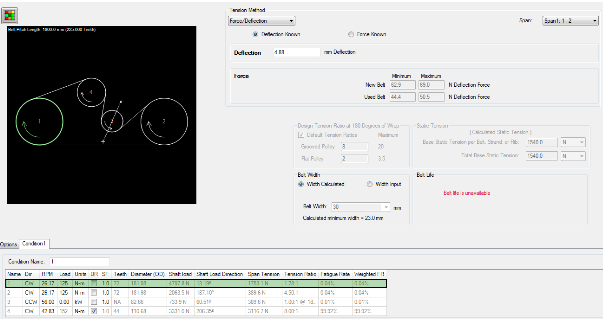
\includegraphics[width=\textwidth]{images/drive_analysis}
\caption[Drive Analysis]{Drive analysis using the Gates Design IQ software.}
\label{fig:drive_analysis}
\end{figure}

\begin{figure}[H]
\centering
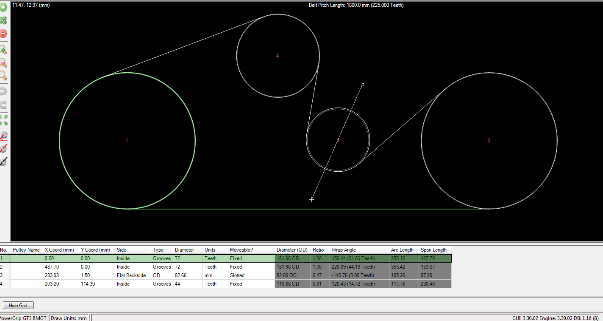
\includegraphics[width=\textwidth]{images/drive_layout}
\caption[Drive Layout]{Drive layout using the Gates Design IQ software.}
\label{fig:drive_layout}
\end{figure}

\subsection{Wheel Shaft}\label{sec:ws_fea}

\begin{figure}[H]
	\centering
	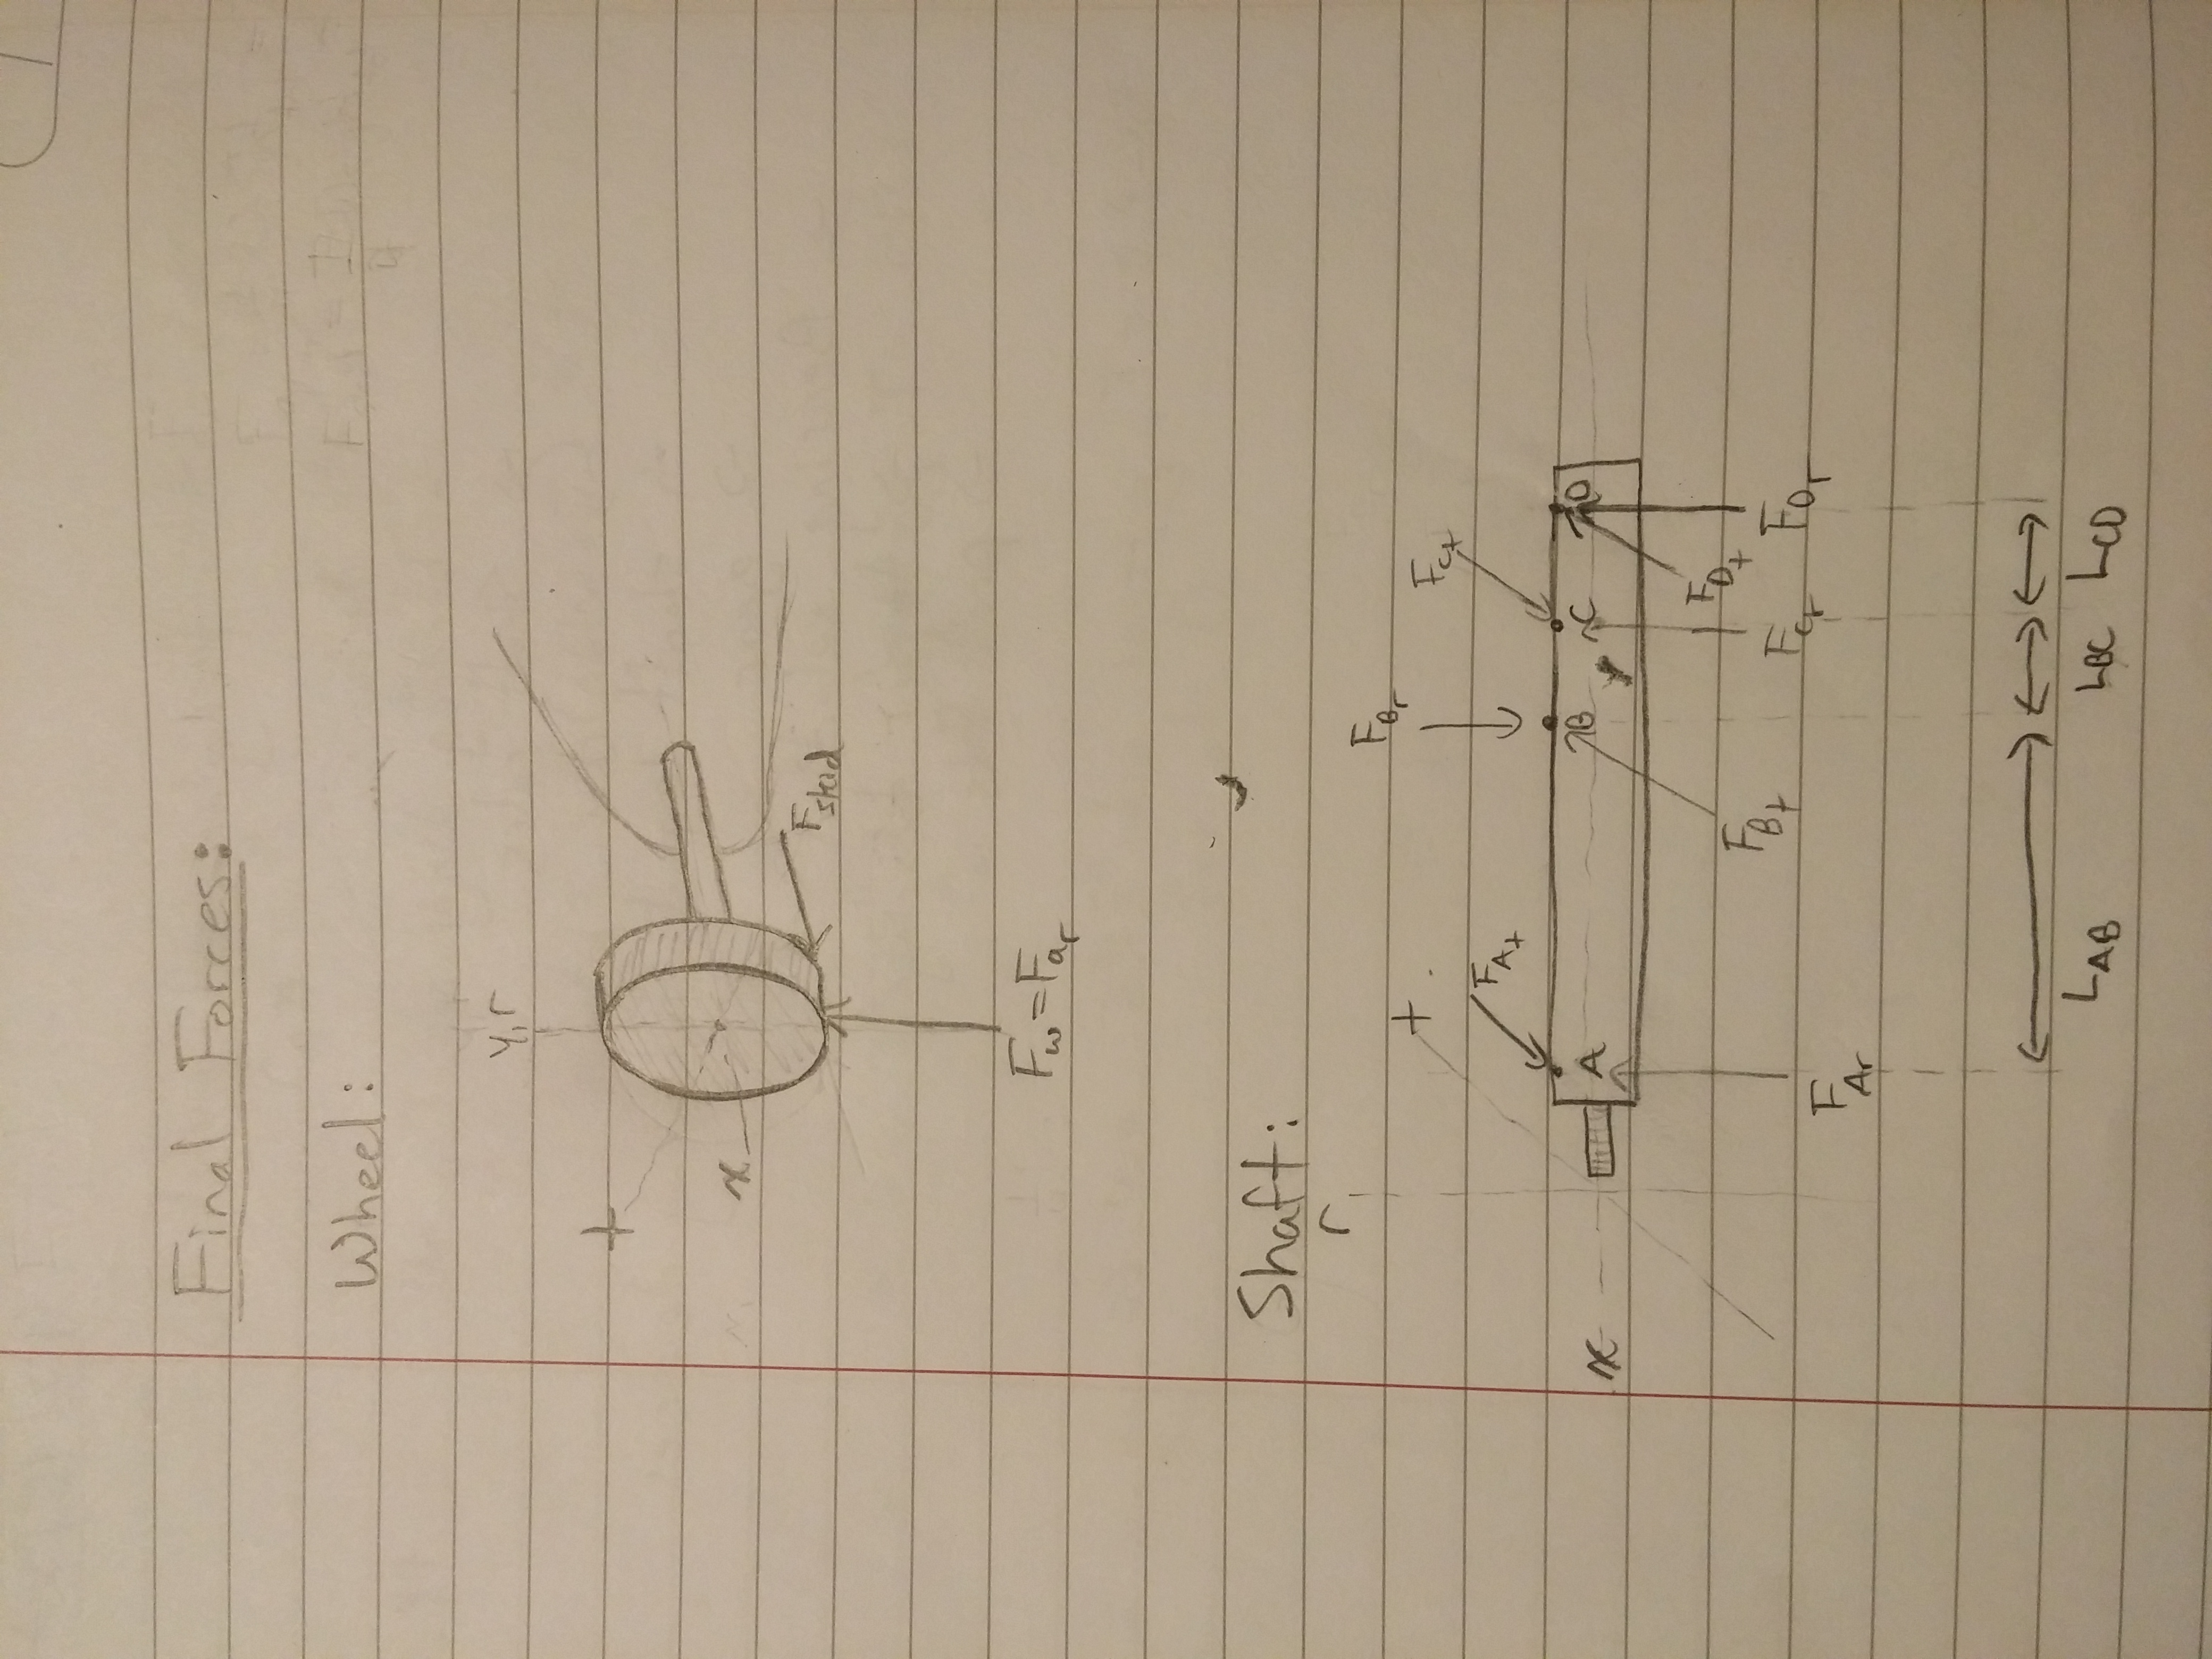
\includegraphics[width=\textwidth,angle=-90]{dom/loading_conditions_calc.jpg}
	\caption{FBD of loading conditions for wheel shaft.}
	\label{fig:fbd_wheelshaft}
\end{figure}

\begin{figure}[H]
\centering
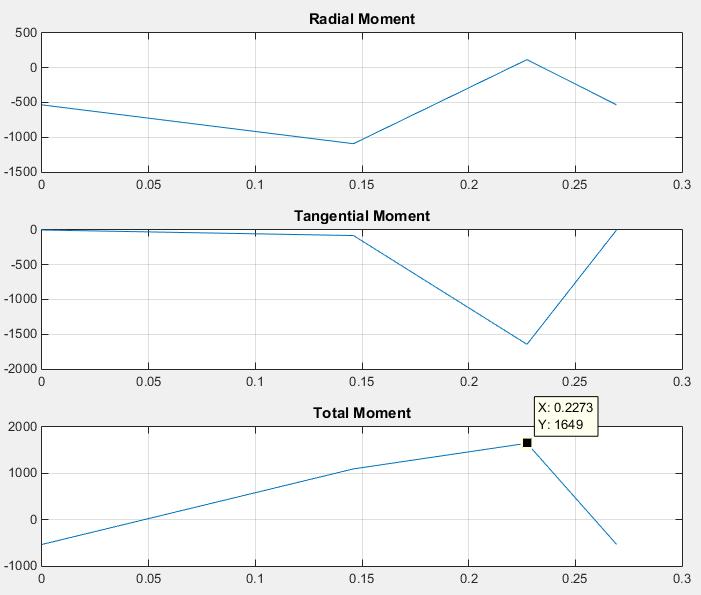
\includegraphics[width=\textwidth]{images/wheelshaft_bmd}
\caption{Wheel Shaft Bending Moment Diagram}
\label{fig:wheel_shaft_bmd}
\end{figure}

\begin{figure}[H]
	\centering
	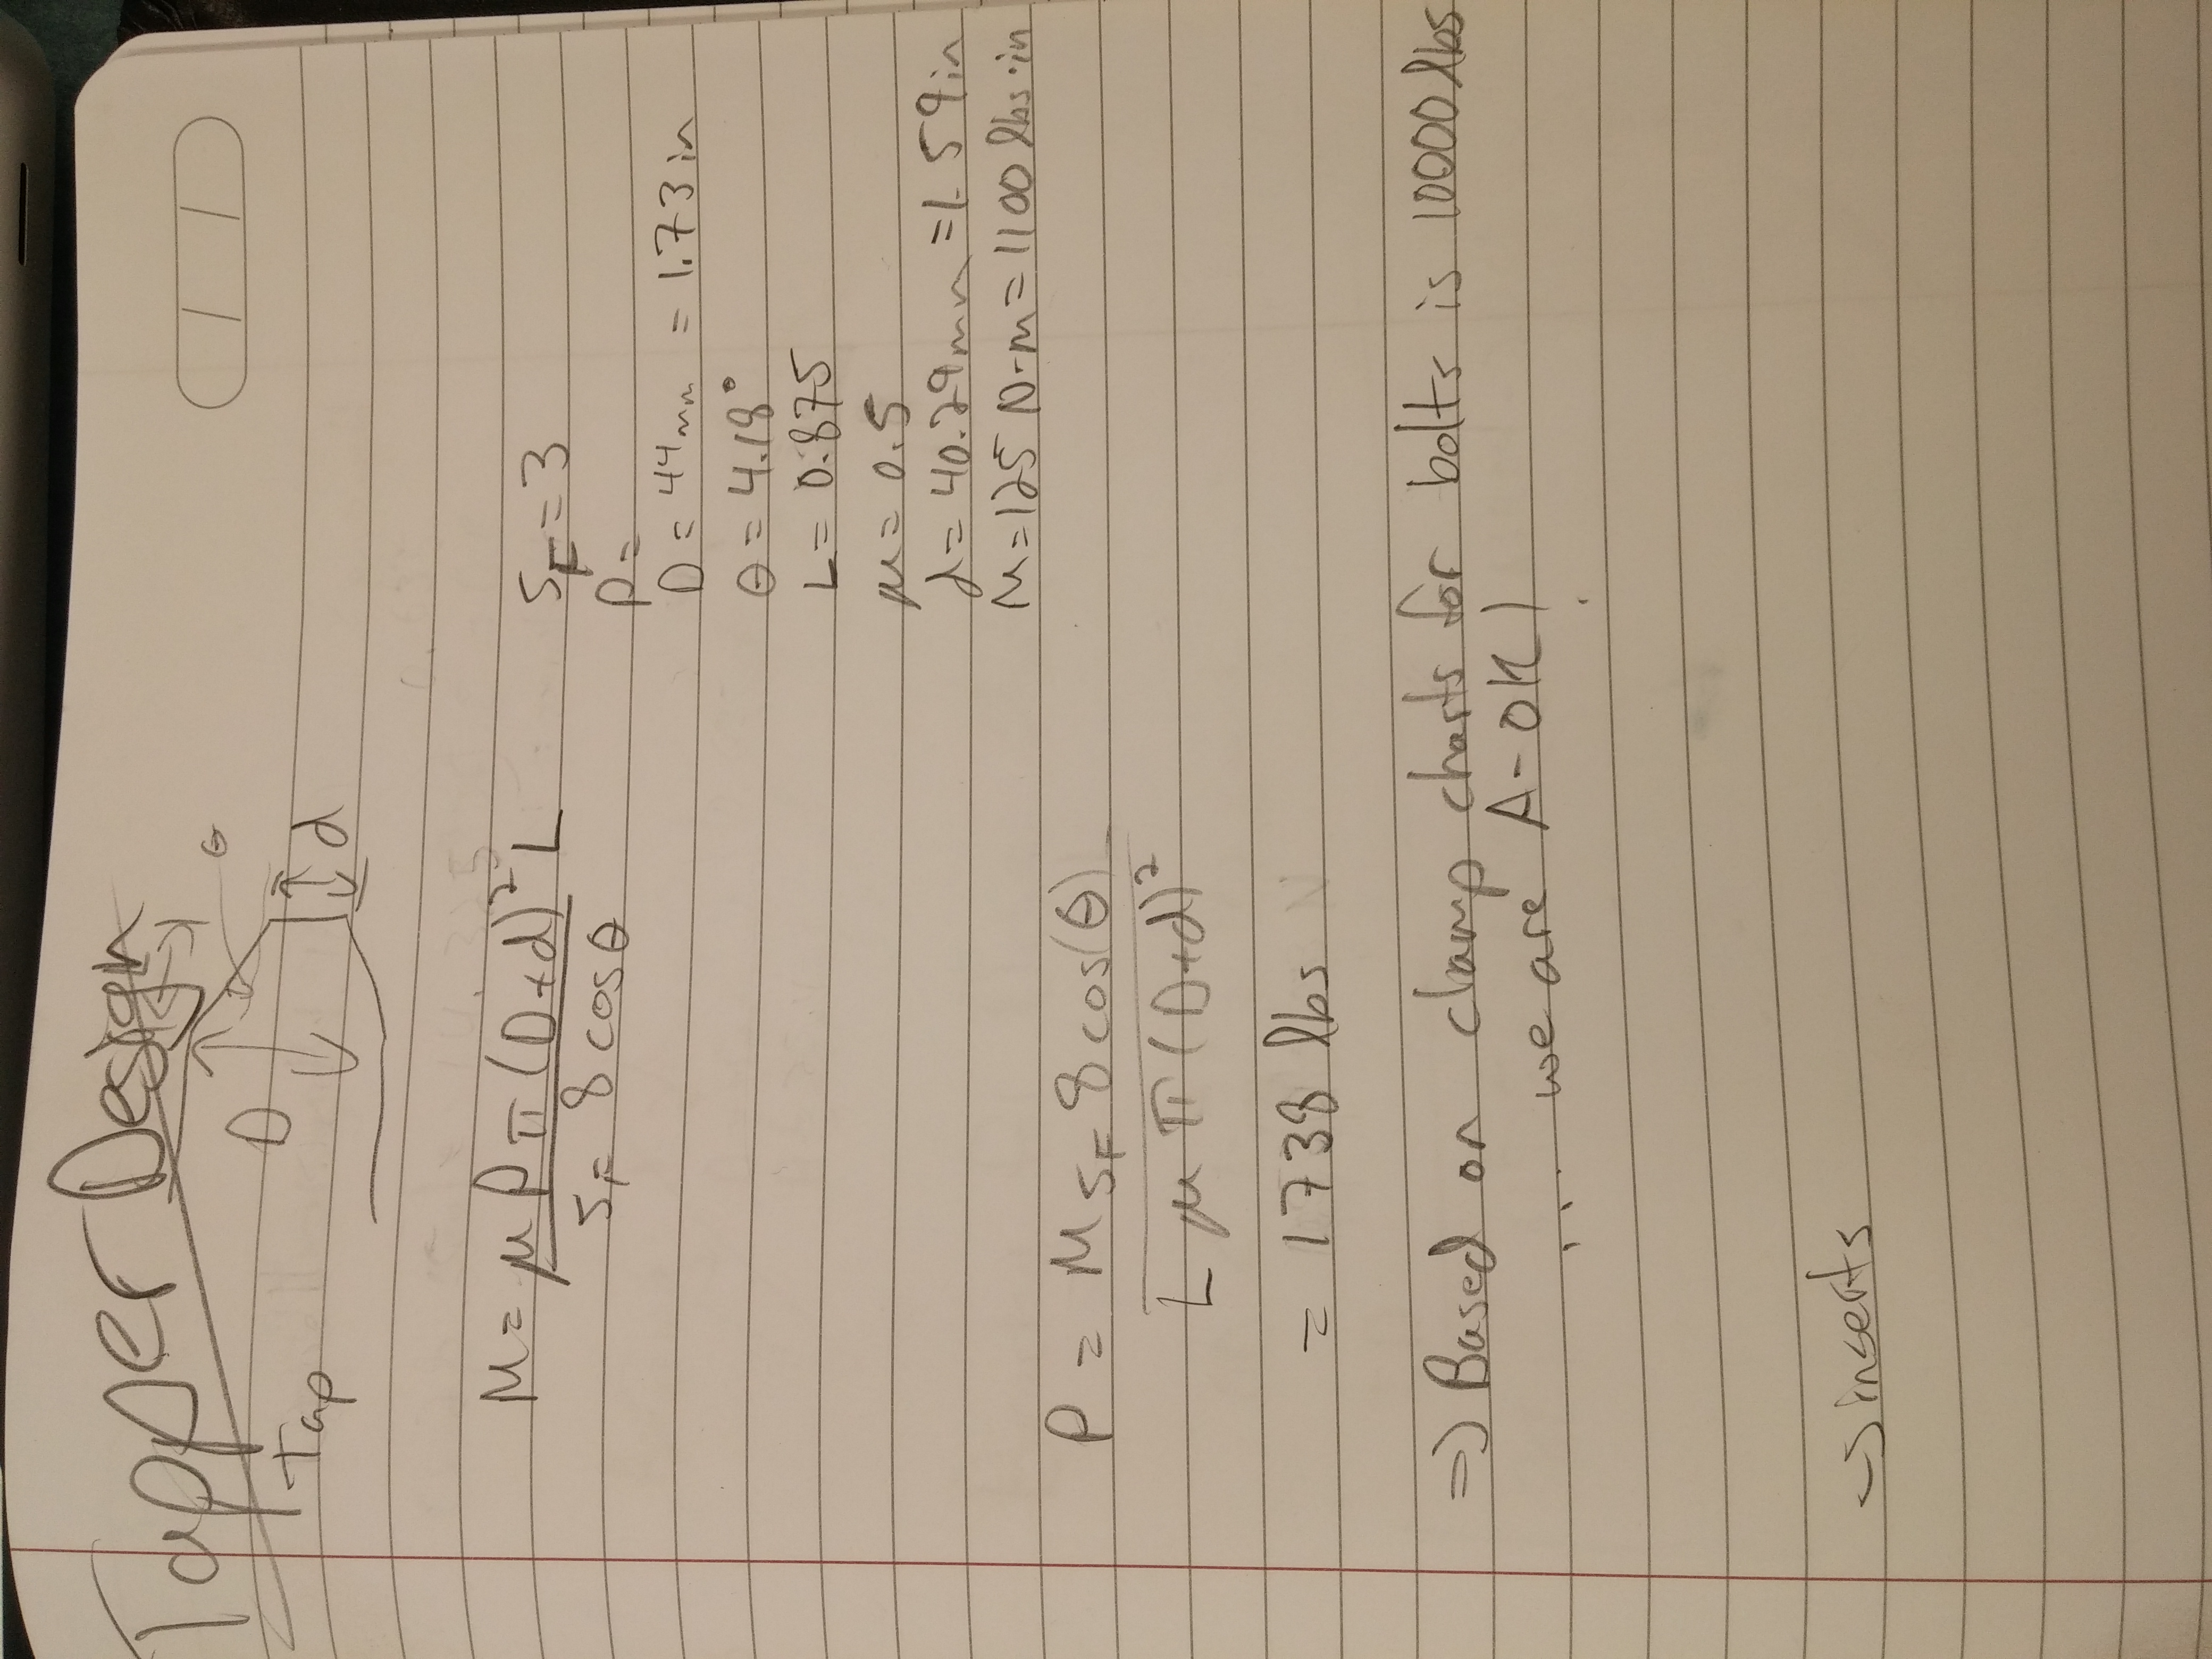
\includegraphics[width=\textwidth,angle=-90]{dom/taper_design_calc.jpg}
	\caption{Taper Mount Design Calculations}
	\label{fig:taper_calc}
\end{figure}

\begin{figure}[H]
\centering
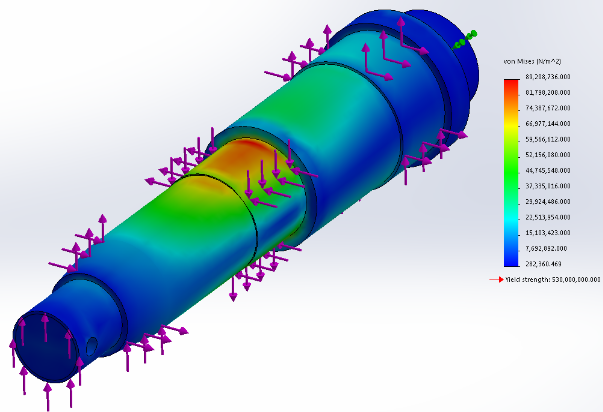
\includegraphics[width=\textwidth]{images/wheel_shaft_fea}
\caption[Wheel Shaft FEA Stress Results]{FEA stress results for wheel shaft. Maximum stress is 81 MPa}
\label{fig:wheel_shaft_stress_fea}
\end{figure}

\subsection{Wheel Bearings}\label{sec:ws_bearing}

\begin{table}[htbp]
	\centering
	\caption{Brief Bearing Selection Table}
	\begin{tabular}{| p{4cm}p{4cm}p{4cm}l |} \hline
		Bearing Type & Pros & Cons & Final Say \\ \hline
		\multirow{2}{4cm}{Deep Groove Ball Bearing} & Sealed & Low Load Capabilities & \multirow{2}{*}{Yes} \\
		& No transferred axial load & Larger outer diameter & \\ \hline
		\multirow{2}{4cm}{Regular Angular Contact Ball Bearings} & \multirow{2}{4cm}{Decent axial loading capabilities} & Poor load capacity & \multirow{2}{*}{No} \\
		& & Need minimum load & \\ \hline
		\multirow{3}{4cm}{Four Point Angular Contact Ball Bearings} & Great load carrying capacity & \multirow{3}{4cm}{Requires axial load larger than radial load} & \multirow{3}{*}{No} \\
		& Thin & & \\
		& Sealed & & \\ \hline
		\multirow{3}{4cm}{Tapered Roller Bearings} & Small & Not sealed & \multirow{3}{*}{Yes} \\
		& Great axial loading capabilities & Imposed axial load from radial load & \\
		& Lightweight & & \\ \hline
	\end{tabular}
	\label{tab:bearing_selection}
\end{table}

\begin{figure}[H]
	\centering
	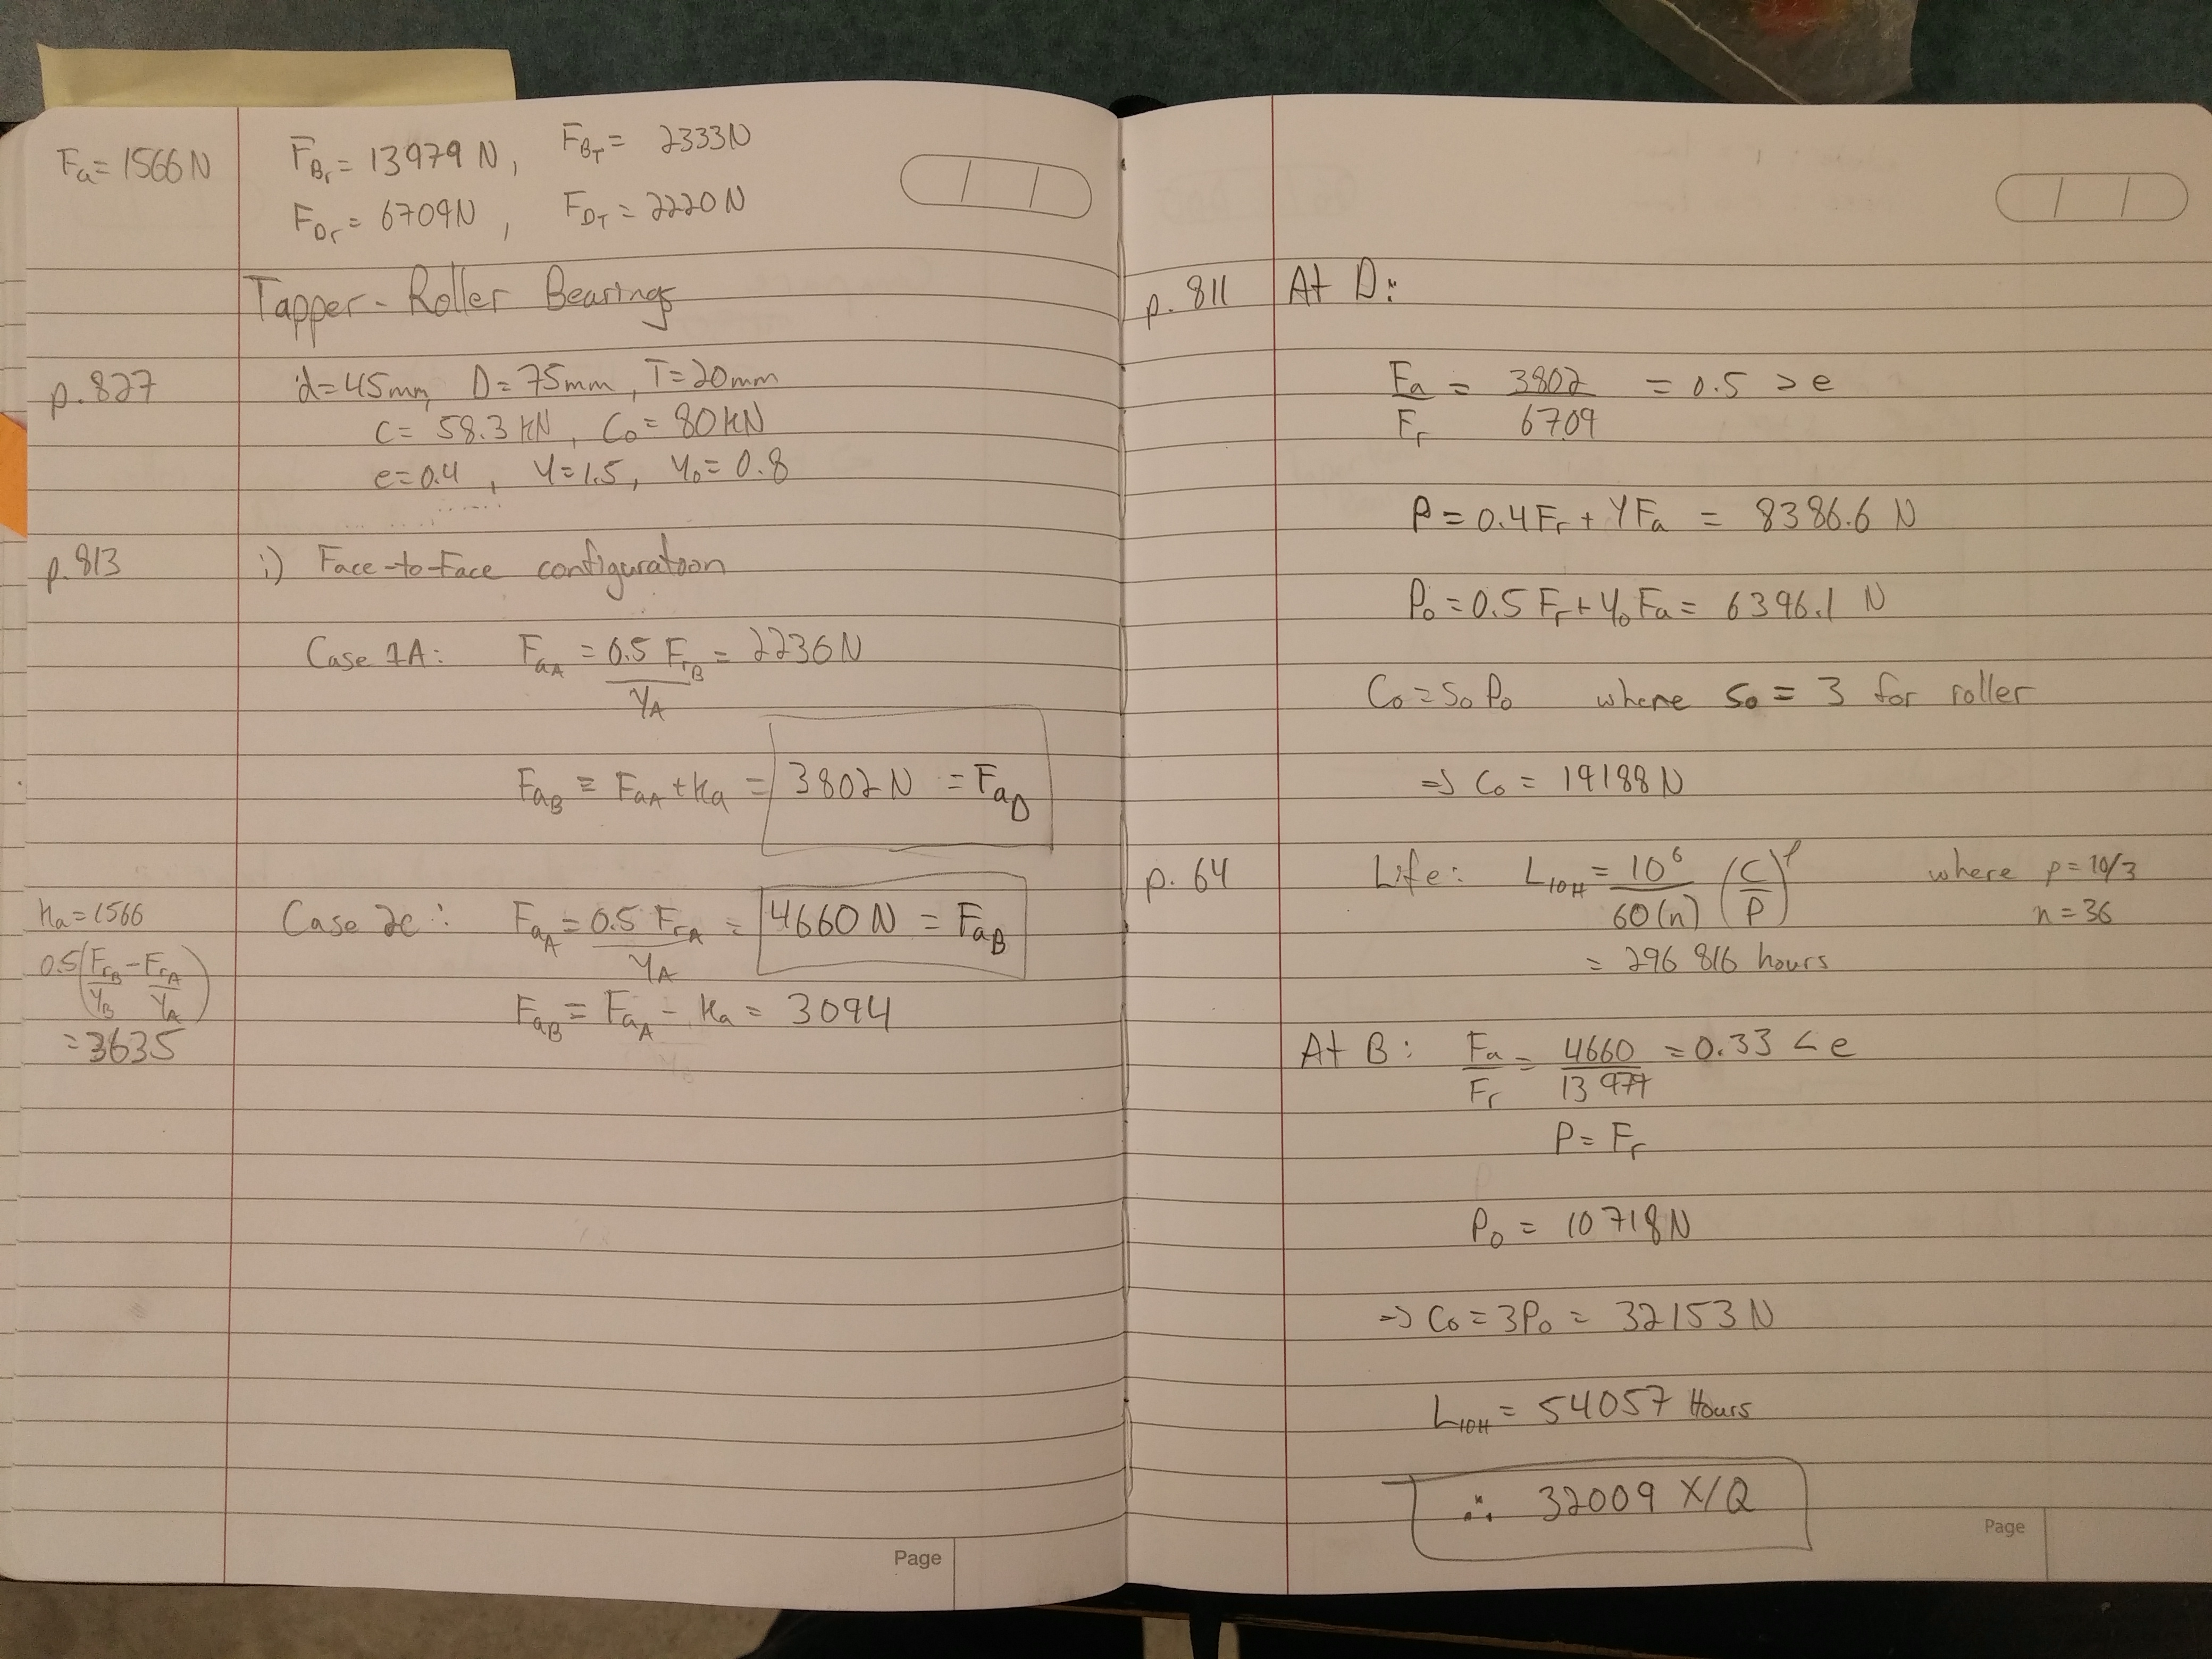
\includegraphics[width=0.8\textwidth]{dom/bearing_selection_calc.jpg}
	\caption{Sample calculation for bearing selection process.}
	\label{fig:bearing_calc}
\end{figure}

\subsection{Bearing Housing}\label{sec:bh_fea}

\begin{figure}[H]
\centering
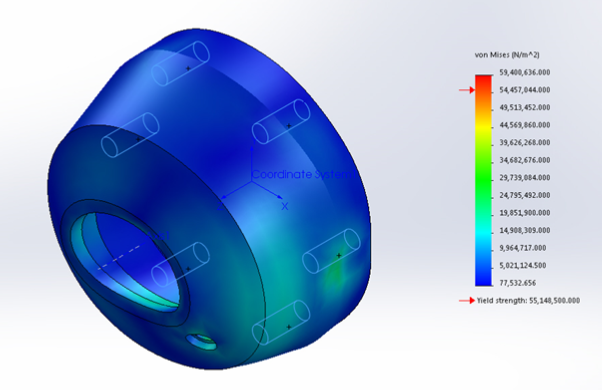
\includegraphics[width=\textwidth]{images/wheel_hub_fea}
\caption[Wheel Bearing Housing FEA Stress Results]{FEA stress results for wheel bearing housing. Maximum stress is 59 MPa}
\label{fig:wheel_hub_stress_fea}
\end{figure}


\subsection{Drive Shaft}\label{sec:drive_shaft_fea}

\begin{figure}[H]
\centering
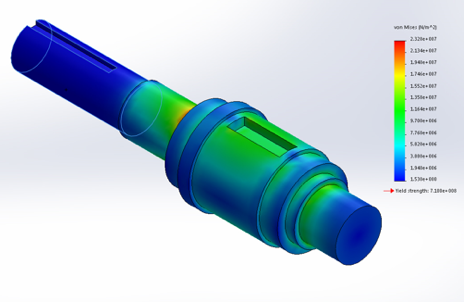
\includegraphics[width=\textwidth]{images/FEA_driveShaft}
\caption[Drive Shaft FEA Stress Results]{FEA stress results for drive shaft. Maximum stress is 23 MPa}
\label{fig:wheel_shaft_stress_fea}
\end{figure}

\subsection{Pivot}\label{sec:pivot_fea}

\begin{figure}[H]
\centering
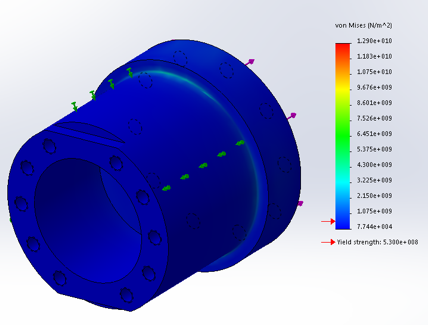
\includegraphics[width=0.9\textwidth]{images/FEA_pivotfinal}
\caption[Pivot FEA Stress Results]{FEA stress results for pivot analysis.}
\label{fig:pivot_stress_fea}
\end{figure}

\begin{figure}[H]
\centering
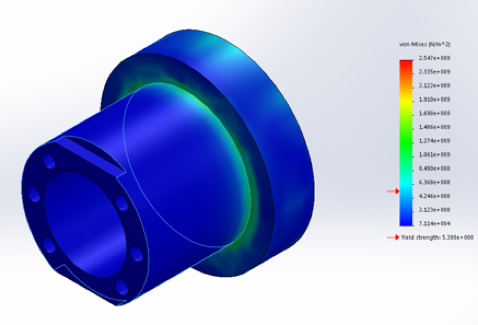
\includegraphics[width=0.9\textwidth]{images/FEA_pivotold}
\caption[Pivot FEA Stress Results]{FEA stress results for pivot analysis.}
\label{fig:old_pivot_stress_fea}
\end{figure}


\subsection{Drive Box}\label{sec:box_fea}

\begin{figure}[H]
\centering
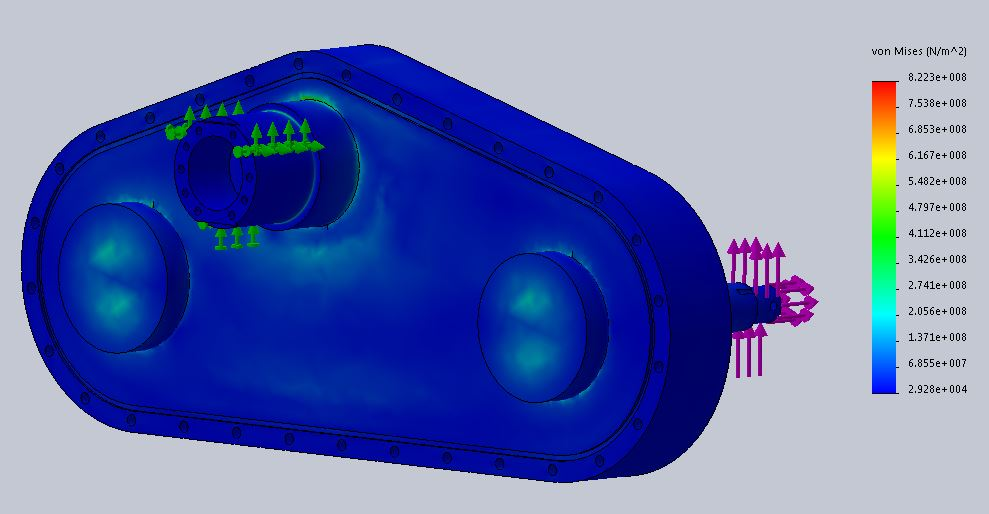
\includegraphics[width=\textwidth]{images/drive_box_stress_fea}
\caption[Drive Box FEA Stress Results]{FEA stress results for drive box analysis. Maximum stress is 82.23 MPa.}
\label{fig:box_fea1}
\end{figure}

\begin{figure}[H]
\centering
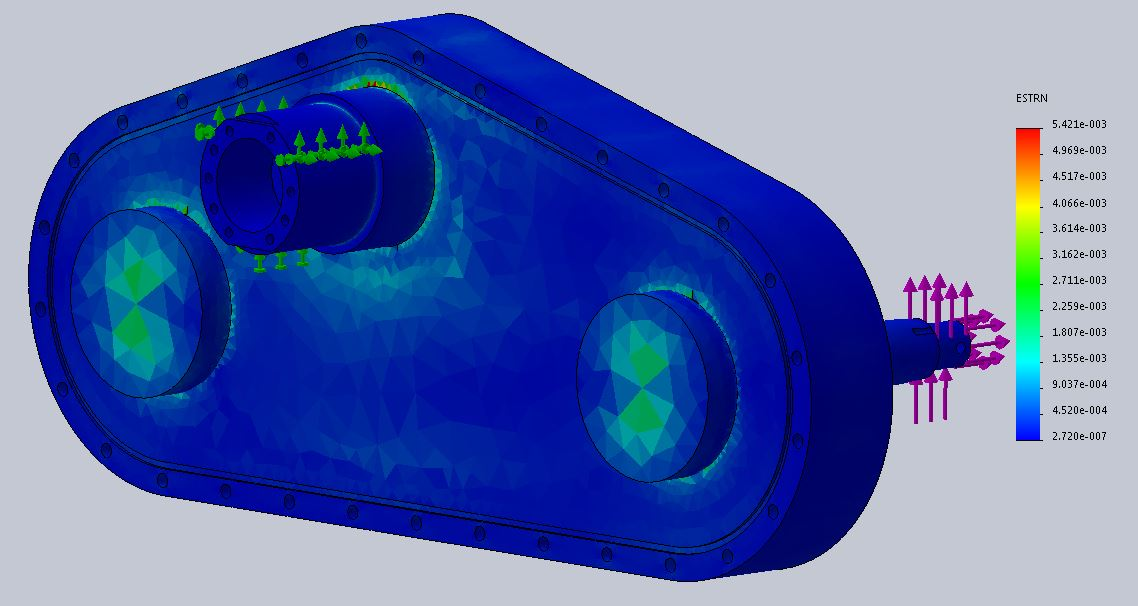
\includegraphics[width=\textwidth]{images/drive_box_strain_fea}
\caption[Drive Box FEA Strain Results]{FEA strain results for drive box analysis. Maximum strain is 5 mm.}
\label{fig:box_fea2}
\end{figure}

\subsection{Tensioner}\label{sec:idler_fea}

\begin{figure}[H]
\centering
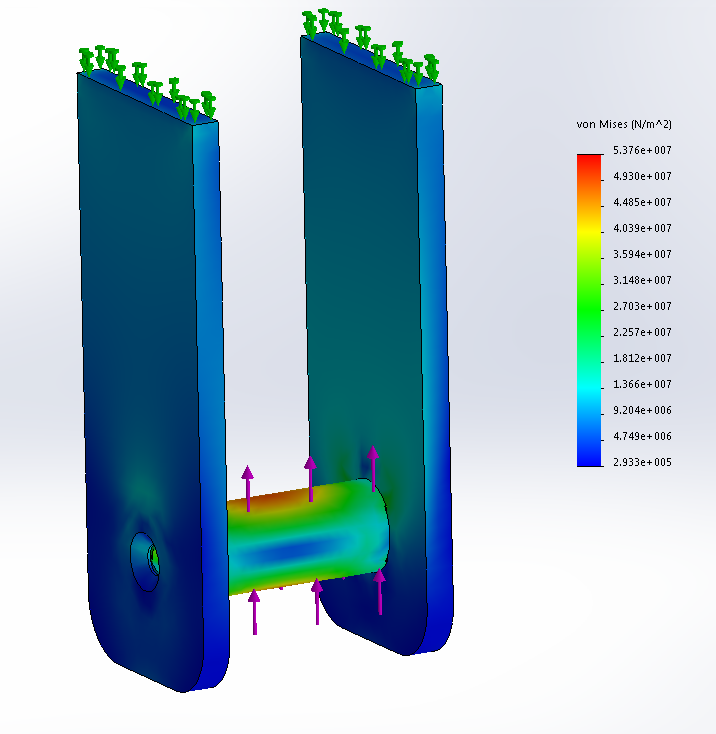
\includegraphics[width=\textwidth]{images/tensioner_vonmises_fea}
\caption[Tensioner FEA Stress Results]{FEA stress results for tensioner analysis. Maximum stress is 53.6 MPa.}
\label{fig:idler_fea1}
\end{figure}

\begin{figure}[H]
\centering
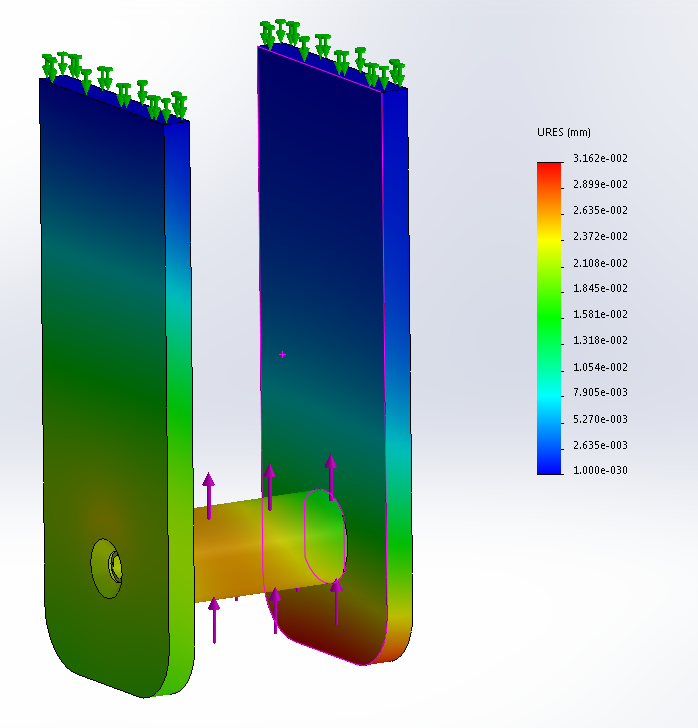
\includegraphics[width=\textwidth]{images/tensioner_displacement_fea}
\caption[Tensioner FEA Displacement Results]{FEA displacement results for tensioner analysis. Maximum displacement is 0.03 mm.}
\label{fig:idler_fea2}
\end{figure}

\subsection{Battery Rack}\label{sec:br_fea}

\begin{figure}[H]
\centering
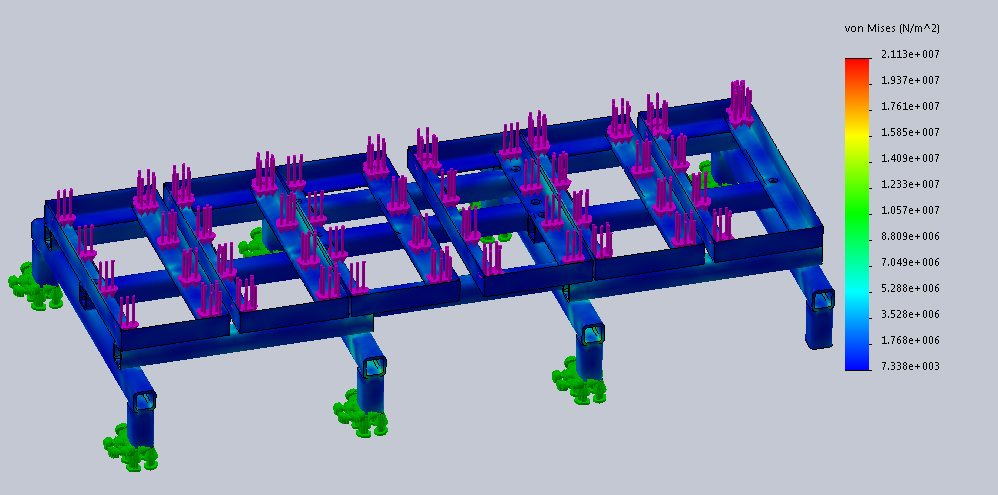
\includegraphics[width=\textwidth]{images/updated_battery_rack_VM}
\caption[Battery Rack FEA Stress Results]{FEA stress results for battery rack analysis. Maximum stress is 21.1 MPa.}
\label{fig:battery_rack_stress_fea}
\end{figure}

\begin{figure}[H]
\centering
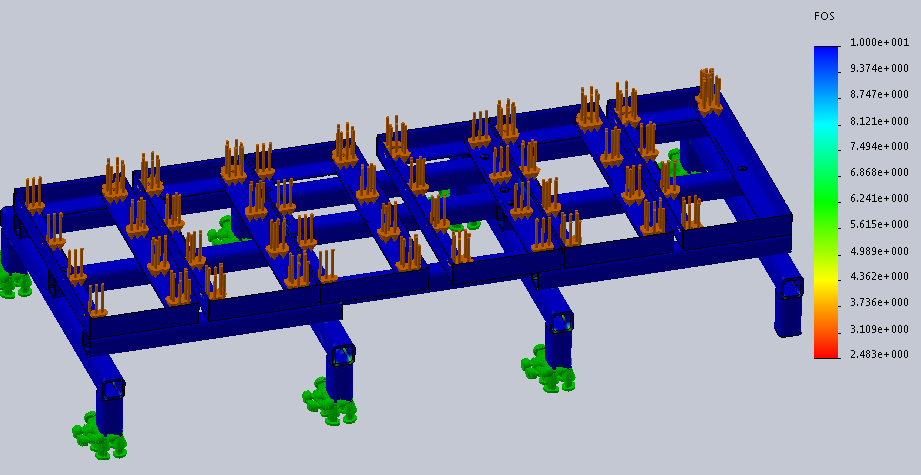
\includegraphics[width=\textwidth]{images/updated_battery_rack_FOS}
\caption[Battery Rack FEA factor of safety Results]{FEA factor of safety results for battery rack analysis. The smallest factor of safety is 2.5.}
\label{fig:battery_rack_disp_fea}
\end{figure}



\section{Excel Tables} \label{excel}

\begin{table}[H]
\centering
\caption{Results of Mass Analysis Performed in Solidworks}
\begin{tabular}{| $l^l^l^l |} \hline
Assembly & Mass kg & Qty & Total kg \\ \hline
Battery Rack End Section & 4.71 & 2.00 &9.43 \\
Battery Rack Mid Section & 4.96 & 1.00 & 4.96 \\
Frame & 120.00 & 1.00 & 120.00 \\
Drive box & 21.50 & 4.00 & 86.00 \\
Motor Mounts (incl. motor and reduction) & 38.18 & 4.00 & 152.73 \\
Pivot & 8.30 & 4.00 & 33.20 \\
Wheel Shafts & 7.80 & 8.00 & 62.40 \\
Batteries & 62.73 & 6.00 & 376.36 \\
Wheels & 13.64 & 8.00  & 109.09 \\
Payload & 227.27 & 1.00 & 227.27 \\
Electrical  & 36.36 & 1.00  & 36.36 \\
Fasteners  & 68.18 & 1.00  & 68.18 \\
Belts & 2.27 & 4.00 & 9.09 \\
Misc.  & 90.91 & 1.00 & 90.91 \\
\rowstyle{\bfseries} &  & Total & 1385.99 \\ \hline
  \end{tabular}
 \label{tab:mass}
\end{table}
 
\begin{table}[H]
\centering
\caption{Tractive Effort Calculation Results}
\begin{tabular}{| llll |} \hline
Name & Variable & Value & Units \\ \hline
Gross Vehicle Weight & GVW & 14047 & N \\
Number of Drive Wheels & NW & 8 & - \\
Weight�on each drive wheel & WW & 1755 & N \\
Radius of wheel/tire & RW & 0.2286 & m \\
Desired top speed & Vmax & 0.833 & m/s \\
Desired acceleration time & Ta & 6.1 & s \\
Maximum incline angle & alpha & 0.1972 & rad \\
Worst working surface & Crr & 0.037 & - \\
Gravitational constant & g & 9.81 & m/s\textsuperscript{2} \\
Resistance factor & RF & 1.15 & - \\
Coefficient of Friction & mu & 0.6 &  \\
Rolling resistance & RR & 519.8 & N \\
Grade resistance & GR & 2752.6 & N \\
Acceleration force & FA & 195.6 & N \\
Total tractive effort & TTE & 3467.9 & N \\
Wheel torque & TW & 911.7 & N-m \\
Wheel torque per wheel &  & 114.0 & N-m \\
Maximum tractive torque & MTT & 240.8 & N-m \\
Torque per wheel for constant speed & T\textsubscript{cs} & 93.5 & N-m \\ \hline
 \end{tabular}
 \label{tab:drivespec}
 \end{table}
 
\section{Work Breakdown Structure}

\begin{figure}[htbp]
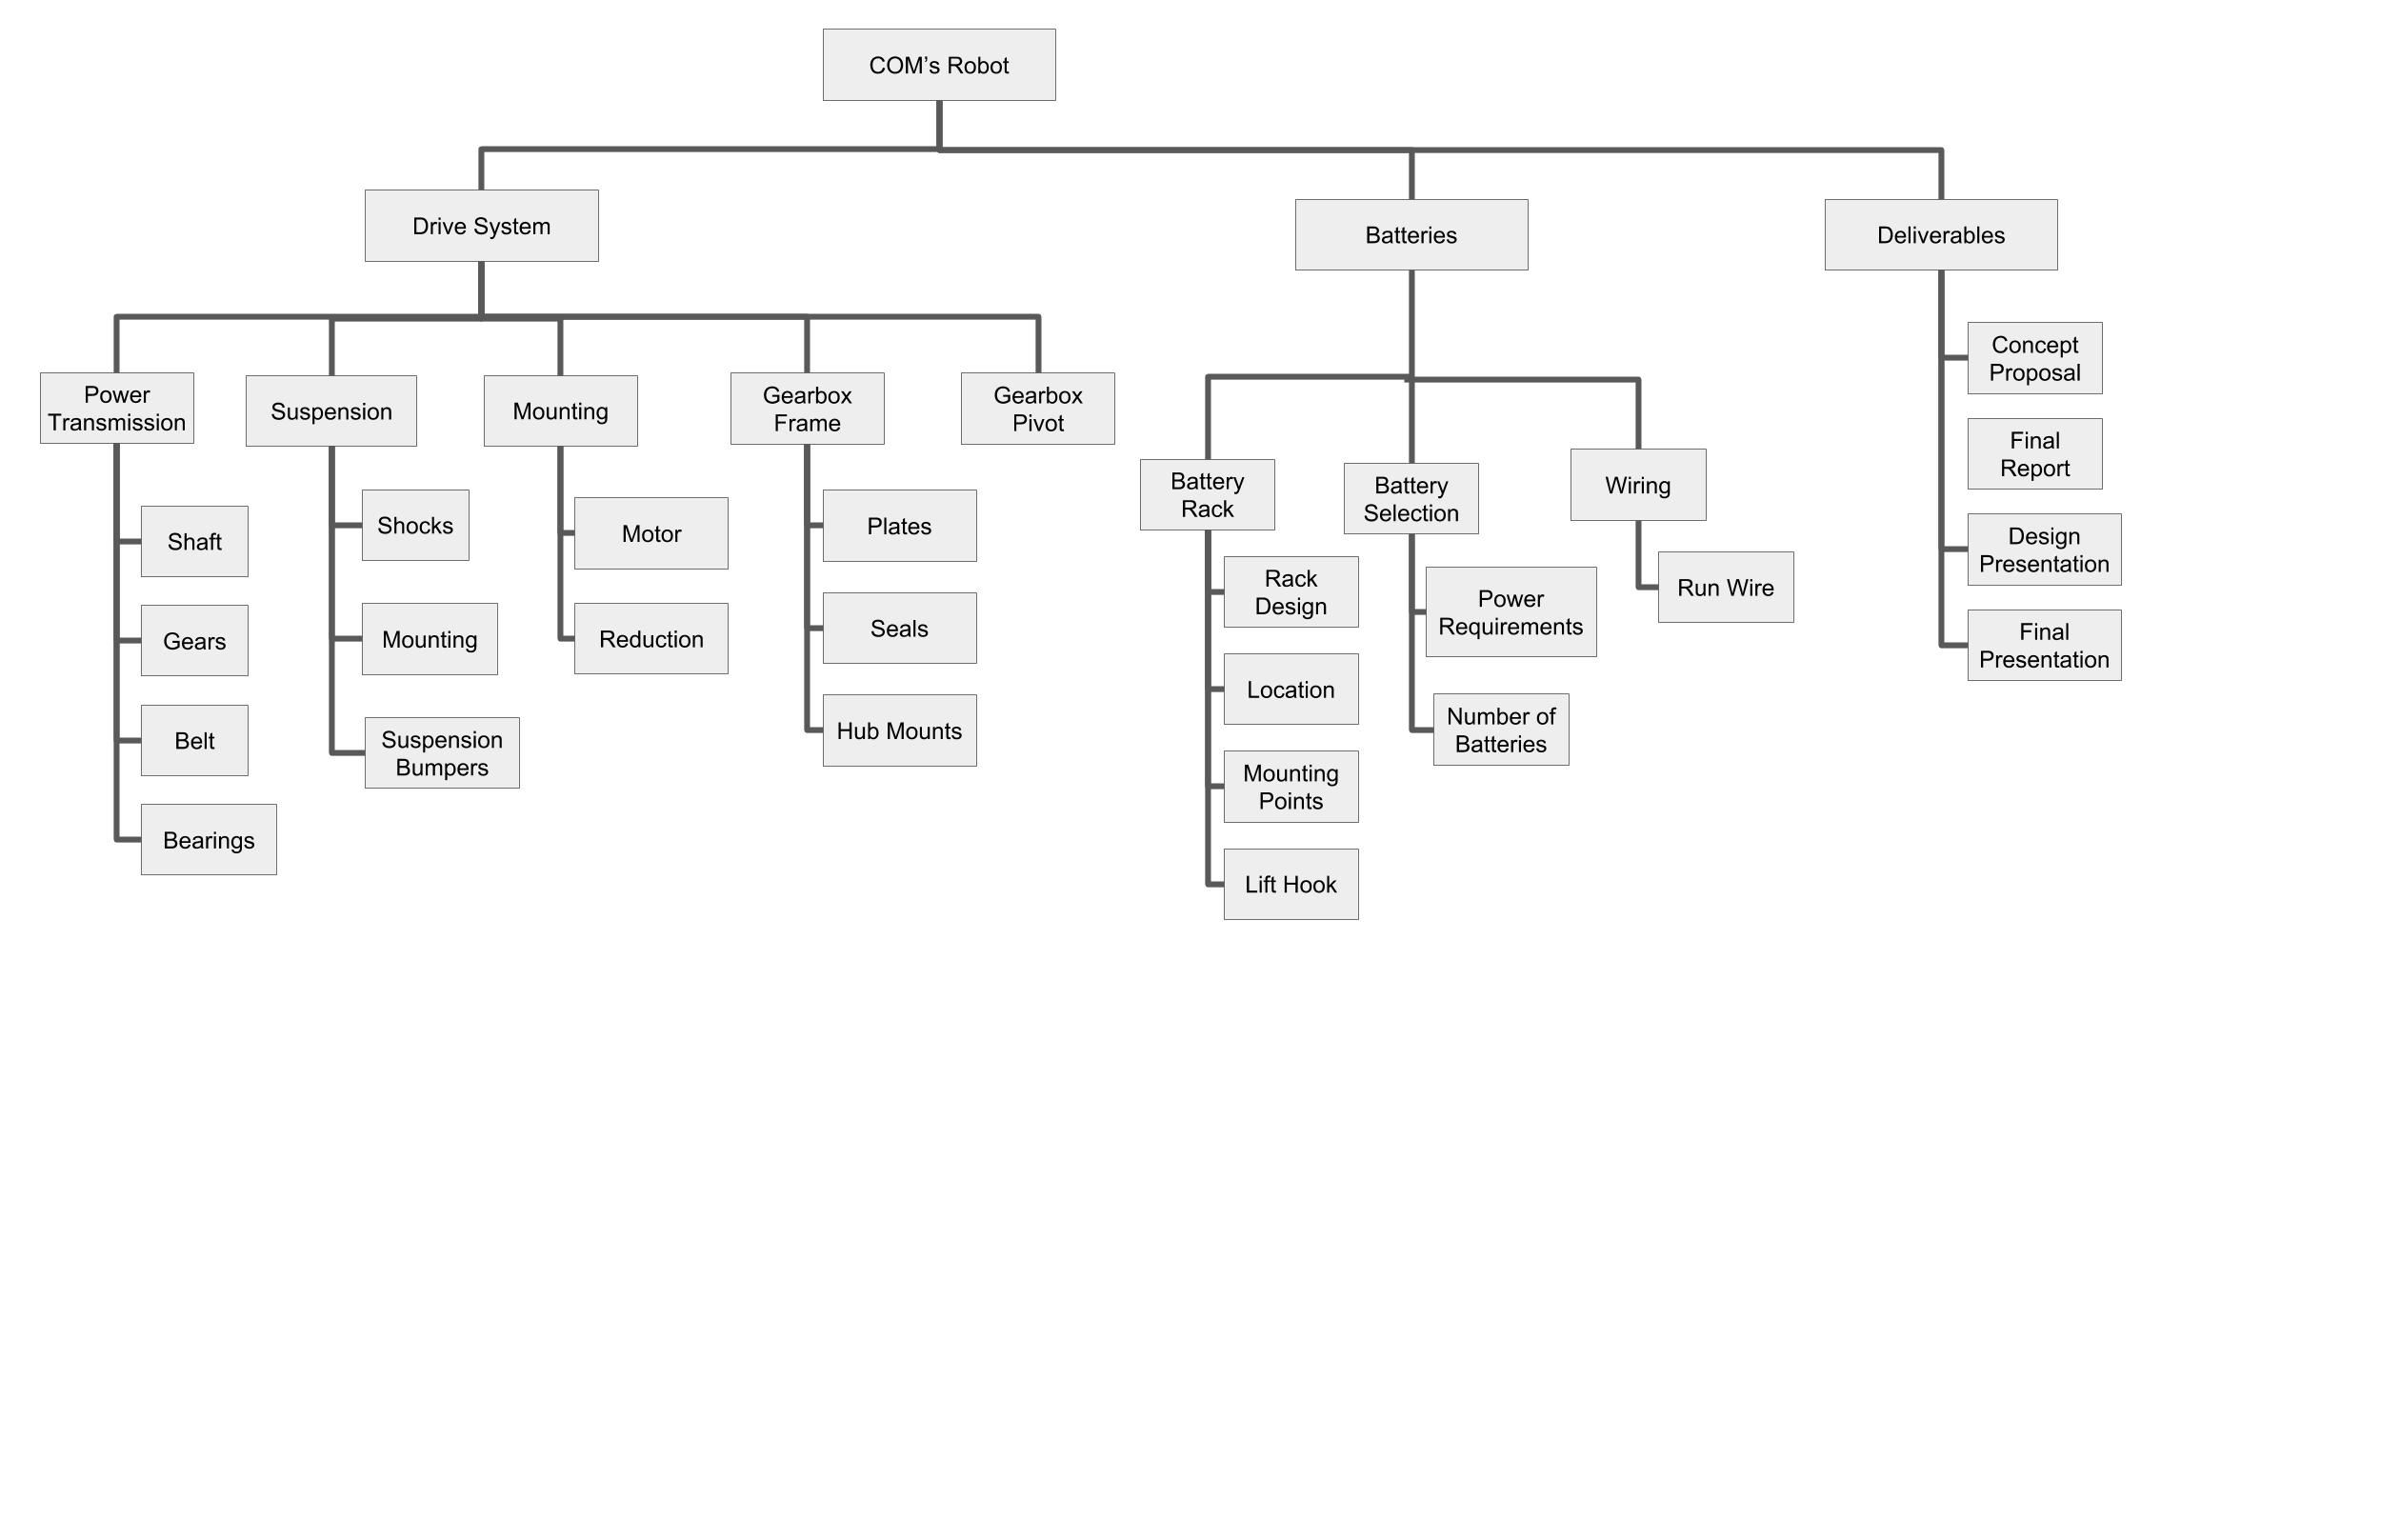
\includegraphics[width=\linewidth]{images/wbs.png}
\caption{Work Breakdown Structure for the project}
\label{fig:wbs}
\end{figure}
\begin{landscape}
\section{DFMEA} \label{dfmea}
\begin{minipage}{\linewidth}
\captionof{table}[DFMEA]{Design Failure Modes and Effect Analysis for Drive Box}
\footnotesize
\begin{tabular}{| p{1cm}|p{3cm}p{3.5cm}p{0.5cm}p{3cm}p{0.5cm}p{3.5cm}p{0.5cm}p{0.5cm}p{3cm} |} \hline
Purpose & Potential Failure Mode & Potential Effects of Failure & SEV & Potential Cause of Failure & OCC & Current Controls Evaluation Method & DET & RPN & Recommended Actions \\ \hline
\multirow{2}{1cm}{Seal} & Plates bend, create gap & Premature wear to belts/reduced belt life & 7 & Plate cannot support robot weight & 4 & O-rings damaged, water in drivebox, belt slip & 9 & 252 & Reinforce plates, check bolt tension \\
& Seals fail & Cause belt slip  & 8 & Deflection in drive box components & 4 & Water inside drivebox, belt slippage & 6 & 192 & Reinforce plates, check bolt tension \\ \hline
\multirow{5}{1cm}{Transmit Torque} & Belt breaks & Vehicle doesn't move & 9 & Sudden tension increase & 3 & Wheels don't turn, vehicle output reduced & 3 & 81 & Replace the belt  \\
 & Belt slips & Vehicle partially moves & 8 & Seals fail & 3 & Vehicle output reduced, less responsive, noise & 6 & 144 & Revise sealing issue \\
 & Bearings too tight, cause friction & Premature wear of bearings & 6 & Improper fitting of bearing & 2 & Wheels don't turn freely & 8 & 96 & Machine to proper tolerance \\
 & Bearings break & Wheels stop rolling, vehicle skids. Damage to belts & 7 & Improper fitting of bearing & 1 & Unwanted noise & 3 & 21 & Replace bearing and observe cause of breaking \\
 & Back plate deforms & Inoperable vehicle & 10 & Material strength too low & 6 & Angled drivebox & 7 & 420 & Reinforce back plate \\ \hline
\multirow{5}{1cm}{Support Robot Weight} & Pivot pierces through back plate & Dysfunctional drivebox & 9 & Plate not thick enough, too much force & 5 & Dragging drivebox, drivebox falls off & 1 & 45 & Redesign back plate \\
 & Plate deflection & Belt snaps, possible break of seal - vehicle cannot drive & 5 & Plate not thick enough too much force & 3 & Snapped belt, visual/angled drivebox & 6 & 90 & Increase radii of plate cutouts \\
 & Wheel shafts deflect & Added stress on bearings & 3 & Excess weight on shaft & 1 & Angled wheels & 2 & 6 & Revise shaft design \\
 & Bushing failure & Drive box dismounts from frame & 7 & Bushing can't handle skid steer & 3 & Play in bushing, drivebox doesn't spin freely, noise & 1 & 21 & Replace bushings \\
 & Fasteners fail at pivot/drivebox interface& Drive box dismounts from pivot & 7 & Skid steer forces greater than estimated & 3 & Dragging drivebox, drivebox falls off & 1 & 21 & Use a higher grade of fastener \\ \hline
 \end{tabular}
 \label{tab:dfmea}
 \end{minipage}
 \end{landscape}

\end{document}